\documentclass[10pt, fleqn, aspectratio=1610,usenames,dvipsnames]{beamer}
% Preamble for `beamer' slides
% -- Preamble --
\usepackage{xcolor}
\usepackage{colortbl}
\usepackage{multicol}
\usepackage{multirow}
\usepackage{starfont}
\usepackage{hyperref}
\usepackage{etoolbox}	% for TOC spacing fix
\usepackage{parskip}
\usepackage[framemethod=tikz]{mdframed}

% reduce spacing between TOC entries
\makeatletter
\patchcmd{\beamer@sectionintoc}
	{\vskip1.5em}{\vskip0.5em}{}{}
\makeatother

% template settings
\usetheme[progressbar=frametitle]{metropolis}
\setbeamertemplate{frame numbering}[fraction]
\useoutertheme{metropolis}
\useinnertheme{metropolis}
\usefonttheme{metropolis}
\usecolortheme{spruce}

\setbeamercolor{background canvas}{bg=white}
\metroset{block=fill}  % formats `block' display
\hypersetup{
    colorlinks=true,
    linkcolor=blue}
    
% left margin width
\setbeamersize
{text margin left=0.5cm, text margin right=0.5cm}

% alignment 
\defbeamertemplate{description item}{align left}{\insertdescriptionitem\hfill}
\setbeamertemplate{description item}[align left]

% customize default block display
\setbeamertemplate{blocks}[rounded][shadow=true]
\setbeamercolor{block body}{bg=mLightBrown!08}

% -- Macros
\newcommand{\fsc}[1]{\normalfont\scshape{#1}}
\newcommand{\ul}{\rule[0.1in]{\textwidth}{0.2mm}\\ \vspace{-8pt}}
\newcommand*\red{\color{red}}
\newcommand*\dgreen{\color{OliveGreen}}

% -- Variable values for title page
\author{}  % will mess up template if commented out
\date{}     % omit or add your your own date, default is `today'

% -- Override errors
\vfuzz=30pt		% suppress Overfull vbox in Outline
\hypersetup{
	pdfpagelayout=SinglePage,
	pdfauthor={janegca},
	pdfsubject={Hellenistic, Medieval Astrology},
    pdfkeywords={astrology, Greek astrology, Hellenistic astrology, Medieval astrology},
    pdfcreator={TeXworks with pdfLatex, beamer}
}
% -- The Title Slide --
\title{Reception: What will or will not be}
\subtitle{Notes and examples on Reception.}
	\institute{ \large These notes are based primarily on Masha'allah's \textsl{On Reception} trans. Robert Hand, ARHAT, 2nd ed. 1998, and \textsl{Six Astrological Treatises by Masha'allah:The Book of Reception} trans. James Holden, AFA, 2009.
	
\vspace{1em}
	
	Masha'allah tells us that we learn, from reception, \textsl{"Whether something will be or not; when it will be if it should come to pass; when it will become apparent that it will not be if it should not come to pass; what prohibits the matter in case it should not be; and through whom, and from whence it should be if it should come to pass."}[RH p1]}

% -- The Presentation Slides --
\begin{document}
% slides are contained in frames
\begin{frame}
\centering
\begin{minipage}{0.75\textwidth}
\titlepage
\end{minipage}
\end{frame}

% table of contents
\AtBeginSection[]{
	\begin{frame}[t, allowframebreaks]{Outline}
		\fontsize{8pt}{5pt}\selectfont
		%\small
   		\tableofcontents[
   	  		currentsection,
   	  		sectionstyle=show/show,
   	  		subsectionstyle=show/show/hide,
   	  		subsubsectionstyle=show/show/show/hide] 
	\end{frame}
}
% -------------------------------------------------------------------------
\section{Reception Basics}
\subsection{Which Chart Elements are Examined?}
\begin{frame}[t]{Which Chart Elements are Examined?}

The following elements of a chart are examined in judging what will or will not be:
\begin{itemize}
\item[$\bullet$] the 5 planets and two luminaries
\item[$\bullet$] the 12 zodiac signs and their domicile rulers
\item[$\bullet$] the signs of  the Exaltations and Falls of the planets
\item[$\bullet$] the applications and separations of the planets by \Conjunction, \Sextile, \Square, \Trine, or \Opposition\ 
\item[$\bullet$] mutual receptions, return of reception, and "the mutual giving of their disposition"
\end{itemize}
\vspace{0.5cm}

The manner in which a planet commits its \textsl{disposition} helps establish if its significations are effected, prohibited, corrupted, rejected or returned.
\end{frame}

\subsection{Applications and Separations by \Conjunction\ or Aspect}

\begin{frame}[t]{Applications and Separations by \Conjunction\ or Aspect}
\begin{block}{}
The faster, lighter planet (A) moves to \textsl{join} (by \Conjunction, \Sextile, \Square, \Trine, \Opposition) a slower, heavier planet (B) and in so doing, \textsl{A} commits his disposition to \textsl{B} and the aspect does not leave off until the two planets are separated.
\end{block}

\begin{mdframed}[backgroundcolor=gray!5, rightmargin=2em, leftmargin=2em]
\textbf{Note:} Robert Hand says \textsl{"there is no separating orb"} ([RH fn4p5]) and so once the two planets are no longer in a partile (exact according to degree) configuration, the matter is done; however, other authors may consider planets to be in aspect as long as one planet is in the light of another.\footnotemark[1]
\end{mdframed}

\begin{block}{}
A planet \textsl{applying to (joining)} another planet indicates \textsl{"what will be"}. 
\end{block}

\begin{block}{}
A planet separating from another planet indicates \textsl{"what has passed away"}.
\end{block}

\footnotetext[1]{A planet's own light extends for 1/2 its orb in front and behind e.g. the \Sun's orb is 30°, its light extends 15° behind and 15° ahead; for \Venus, whose orb is 16°, her light extends 8° behind and 8° ahead, etc. This concept is the basis of the traditional astrologer's use of \href{https://www.skyscript.co.uk/aspects.html\#mo}{moiety of orb}.}

\end{frame}
\subsection{Committing Disposition}
\begin{frame}[t]{Committing Disposition}
\small
\begin{block}{}
\textbf{Axiom:} Any planet (A) joining another (B) from B's domicile or exaltation \textsl{commits its disposition} to \textsl{B}, who, because of reception, will perfect the matter signified by \textsl{A}.
\end{block}

The language used here makes sense in that if \textsl{A} is in a domicile of \textsl{B} he is a guest in \textsl{B}'s home. Astrologically speaking, the ruler of the domicile (B) is responsible for \textsl{settling} or \textsl{disposing} of all matters within his domicile, including those of other planets lodged there.

The nature of the aspect qualifies the nature of the request as a hard one (\Square, \Opposition), an easy one (\Sextile, \Trine), or a familiar, or congenial, one (\Conjunction).

\textbf{Example:}
\begin{columns}[T, onlytextwidth]
\column{0.25\textwidth}
\Sun\ 10 \Aries\ $\Rightarrow$ \Square\ \Mars\ 10 \Capricorn

\column{0.01\textwidth}
\rule{.1mm}{.27\textheight}

\column{0.75\textwidth}
the \Sun\ applies to the \Square\ of \Mars, \\
committing his disposition to \Mars, who  \\
receives the \Sun\ in his domicile (\Aries), and so \\
\textsl{accepts} the \Sun's disposition and will perfect it, but \\
due to the \Square\, \\ 
only after some anxiety and errors i.e. not easily
\end{columns}
\end{frame}
% -------------------------------------------------------------------------------------------------
\subsubsection{Committing Disposition - Another Example}
\begin{frame}[t]{Committing Disposition - Another Example}
\textbf{Example:}\footnotemark[1]
\begin{columns}[T, onlytextwidth]
\column{0.25\textwidth}
\Sun\ 1 \Libra\ $\Rightarrow$ \Opposition\ \Saturn\ 25 \Aries

\column{0.01\textwidth}
\rule{.1mm}{.20\textheight}

\column{0.75\textwidth}
the \Sun\ is in the Exaltation of \Saturn\ (\Libra) \\
\Saturn\ is in the Exaltation of the \Sun\ (\Aries), therefore \\
there is \textbf{Mutual Recption} by \textsl{exaltation}, and \\
the \Sun\ commits his disposition to \Saturn, who accepts it
\end{columns}
\vspace{0.5cm}
According to Masha'Allah, when there is Mutual Reception, \textsl{"there is peace and the matter will be perfected"}; however, if \Saturn\ leaves \Aries\ before the \Opposition\ can perfect, \textsl{"there will be enmities, contrariness, misunderstandings, denials and \Saturn\ will not receive the \Sun"} and so will not take on the \Sun's disposition.

\footnotetext[1]{The examples used by Masha'Allah so far involve planets in their sign of Fall or Detriment which we will see (in later examples), may result in a commitment being rejected.}
\end{frame}

\subsection{The Joining of Planets}
\begin{frame}[t]{The Joining of Planets}
\begin{block}{}
 Planets are \textsl{joined together} (connected) by recognized aspects (\Sextile, \Square, \Trine, \Opposition) or bodily \Conjunction's that are within orb and will eventually become \textsl{exact by degree}.
 \end{block}
\textbf{Benefics joined to Benefics}\footnotemark[1]

A benefic (\Venus\ or \Jupiter) joined to another benefic is good; if there is also reception, the good indicated by the planets is increased.

\textbf{Benefics joined to Malefics}

If a benefic (\Venus\ or \Jupiter) joins with and is received by a malefic planet (\Mars\ or \Saturn) then the malefics are at peace and \textsl{"their evil goes away"} unless they are joined by a \Square\ or \Opposition, in which case there will be some labour, and error.

\textbf{Malefics joined to Malefics}

If a malefic (\Mars\ or \Saturn) joins with another malefic with reception, they are made good and their evil and impediment goes away. Ibn Ezra says they can receive each other by \Conjunction, \Sextile, or \Trine\  \textsl{``but not in the other aspects''} (p.124)
\vspace{0.5cm}

\footnotetext[1]{Based on the essential nature of the planets; need to check their actual condition in the chart.}
\end{frame}
\subsection{What Constitutes Reception?}
\begin{frame}[t]{What Constitutes Reception?}
\small
\begin{block}{}
\textsl{Reception} happens when one planet (A) is in the domicile or exaltation of another planet (B) whom it aspects or conjuncts. The aspect (or conjunction) from planet \textsl{A} must \textsl{perfect} (become exact)  before planet \textsl{B} moves into another sign or a third planet (C) intercedes by completing its own aspect or conjunction with planet \textsl{B}.
\end{block}

While Masha'allah appears to have been the first to begin categorizing and explaining the way reception, applications, and separations indicate outcomes Sahl ibn Bishr al-Israili (786-845) seems to have been the first to spell out the 16 distinct modes of the "perfection and destruction of things". These were also listed and amplified by  Abu Ma'shar (787-886),  and Ibn Ezra (1089-1164).

Examples from these authors are used to name and describe the various ways in which reception can occur. The referenced texts are:
\begin{itemize}
\small
\item \textsl{The Introduction to the Science of the Judgments of the Stars} by Sahl ibn Bishr trans. James Holden, AFA, 2008 
\item \textsl{The Astrology of Sahl B. Bishr Vol. I} trans. Ben Dykes, Cazimi Press, 2019

\item \textsl{The Abbreviation of the Introduction to Astrology} by Abu Ma'shar trans. Charles Burnett, ARHAT, 2nd. printing, 2000

\item \textsl{Ibn Ezra: The Beginning of Wisdom} trans. Meira Epstein, ARHAT, 1998
\end{itemize}

\end{frame}
% -------------------------------------------------------------------
\subsubsection{Perfect Reception - Pusing Nature}
\begin{frame}[t]{What Constitutes Reception - Perfect Reception: Pushing Nature}
\vspace{0.1cm}
\begin{columns}[T, onlytextwidth]
\column{0.5\textwidth}
An example of \textbf{perfect reception} (according to Sahl) is a planet (A) applying to the domicile or exaltation ruler (B) of the sign it occupies. Ibn Ezra (p121) says the ruler (B) "will confer its nature upon" planet A but other authors say A pushes B's nature onto B.  \\
\vspace{0.2cm}
\textbf{Example (A $\Rightarrow$ B): \Moon\ in \Aries\ $\Rightarrow$ \Mars\ or \Sun} 
\ul
\vspace{0.2cm}
\Moon\ in \Aries\ applying to either of \\
\Mars\ (domicile ruler of \Aries) or \\
\Sun\ (exaltation ruler of \Aries) \\
\vspace{0.2cm}
\Mars\ or the \Sun\ can be in any sign; they receive the \Moon, accepting her disposition, because she is in \Aries\ which \Mars\ rules by domicile and the \Sun\ by exaltation.\\

\column{0.5\textwidth}

\begin{center}
{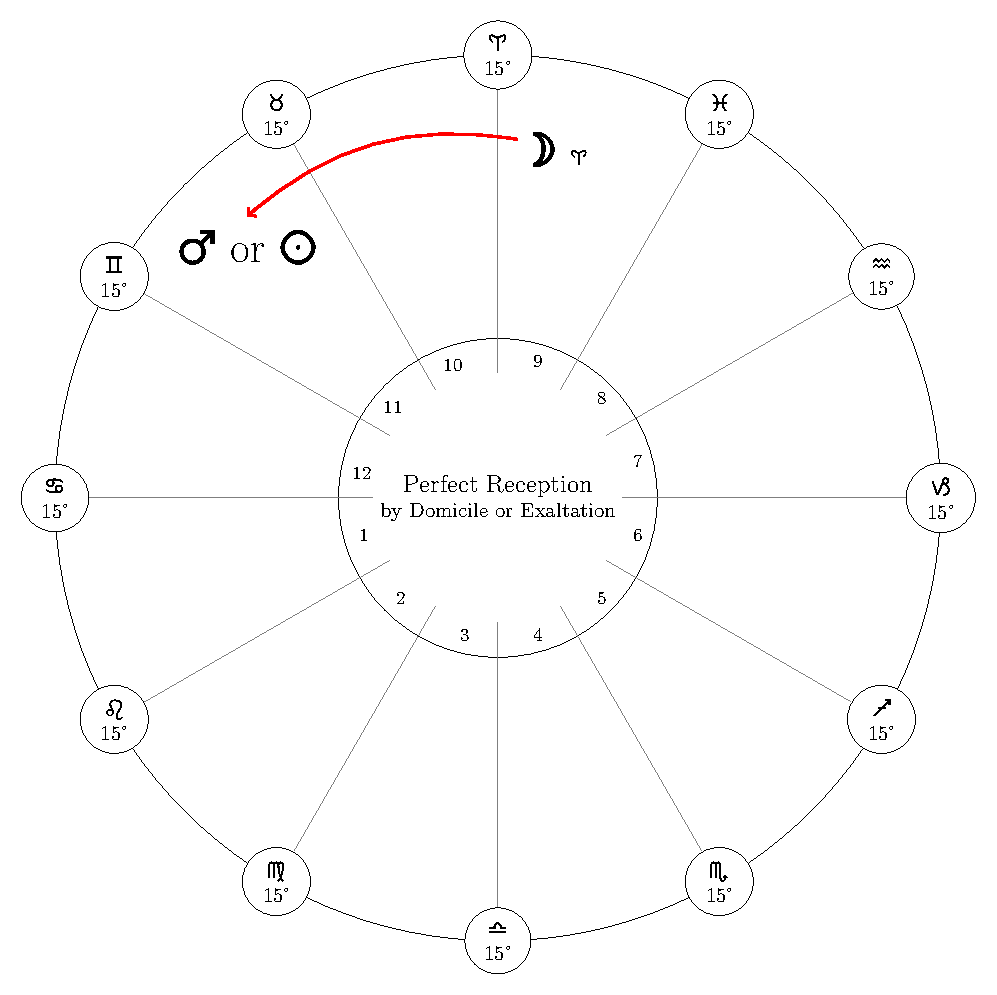
\includegraphics[width=0.8\textwidth]{charts/01-perfect-reception}} \\
\end{center}

\end{columns}
\vspace{0.2cm}
\footnotetext[1]{Sahl, p.18}
\end{frame}
% ----------------------------------------------------
\subsubsection{A Weaker Reception - Pushing Power}
\begin{frame}[t]{What Constitutes Reception - A Weaker Reception: Pushing Power}
\begin{columns}[T, onlytextwidth]
\column{0.5\textwidth}
A planet in its own domicile or exaltation applying to another planet is said by Abu Ma'shar to \textsl{"push [its] power"} to the other planet. Ibn Ezra calls it \textsl{"conferring influence"}; Sahl, \textsl{"giving virtue" or "committing disposition"}.\footnotemark[1]This too is a form of reception but it is considered weaker than perfect reception. Here, \textsl{A} gives his own authority and resources to \textsl{B}. \\
\vspace{0.2cm}
\textbf{Example (A $\Rightarrow$ B):} \Mars\ or \Sun\ in \Aries\ $\Rightarrow$  \Saturn \\
\ul
\vspace{0.2cm}
\Mars\ or \Sun\ in \Aries\ applying to  \\
\Saturn\ in any sign \\
\vspace{0.25cm}
Note that strictly speaking Sahl would consider this a 'non-reception' as \Aries\ is \Saturn's Fall.\footnotemark[2] Other authors accept it as a corrupted reception.

\column{0.5\textwidth}
\begin{center}
{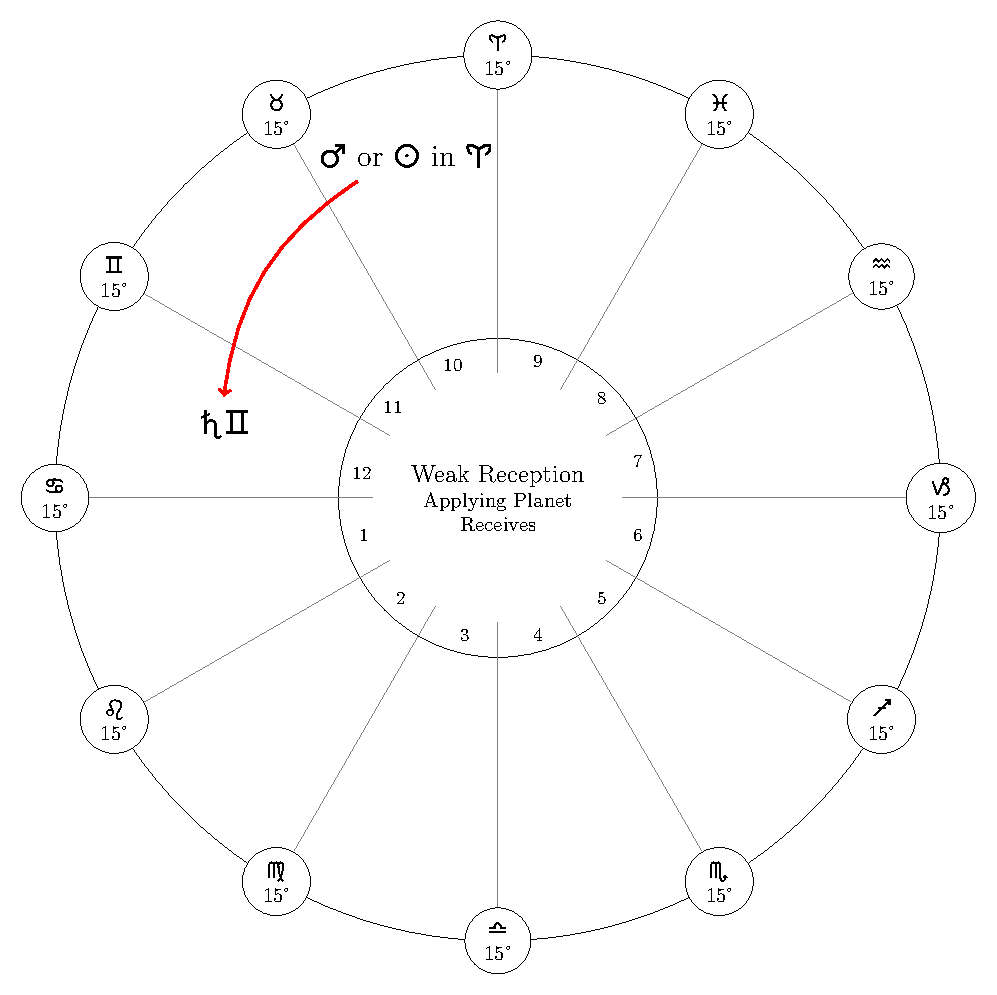
\includegraphics[width=\textwidth]{charts/01-weaker-reception}} \\
\end{center}

\end{columns}
\vspace{0.2cm}
\footnotetext[1]{Abu Ma'shar, p.25;Ibn Ezra, p. 121; Sahl p20 Holden}
\footnotetext[2]{Sahl, Dykes trans. p.62; Holden's, p.19}
\end{frame}
% -------------------------------------------------
\subsubsection{Pushing Two Natures}
\begin{frame}[t]{What Constitutes Reception - Pushing Two Natures}
\begin{columns}[T, onlytextwidth]
\column{0.5\textwidth}
When a planet (A) in its domicile or exaltation applies to another planet (B) who also has dignity in \textsl{A's} place \textsl{A} is said to be "pushing two natures" onto \textsl{B}; his own and \textsl{B}'s.\footnotemark[1]\\
\vspace{0.2cm}
\textbf{Example (A $\Rightarrow$ B):} \Venus\ in \Pisces\ $\Rightarrow$ \Jupiter \\
\ul
\Venus\ exalted in \Pisces\ applies to \\
\Jupiter\ who is the domicile ruler of \Pisces \\
\Venus\ pushes her own and \Jupiter's nature, onto \Jupiter \\
\vspace{0.2cm}

Rob Hand also describes another form of reception called \textbf{communion} which happens when two planets are found in the same sign with one ruling the sign and the other being the exaltation ruler of the sign e.g. \Moon\ and \Jupiter\ both in \Cancer, or \Mars\ and \Sun\ both in \Aries, etc.

\column{0.5\textwidth}
\vspace{-0.5cm}
\begin{center}
{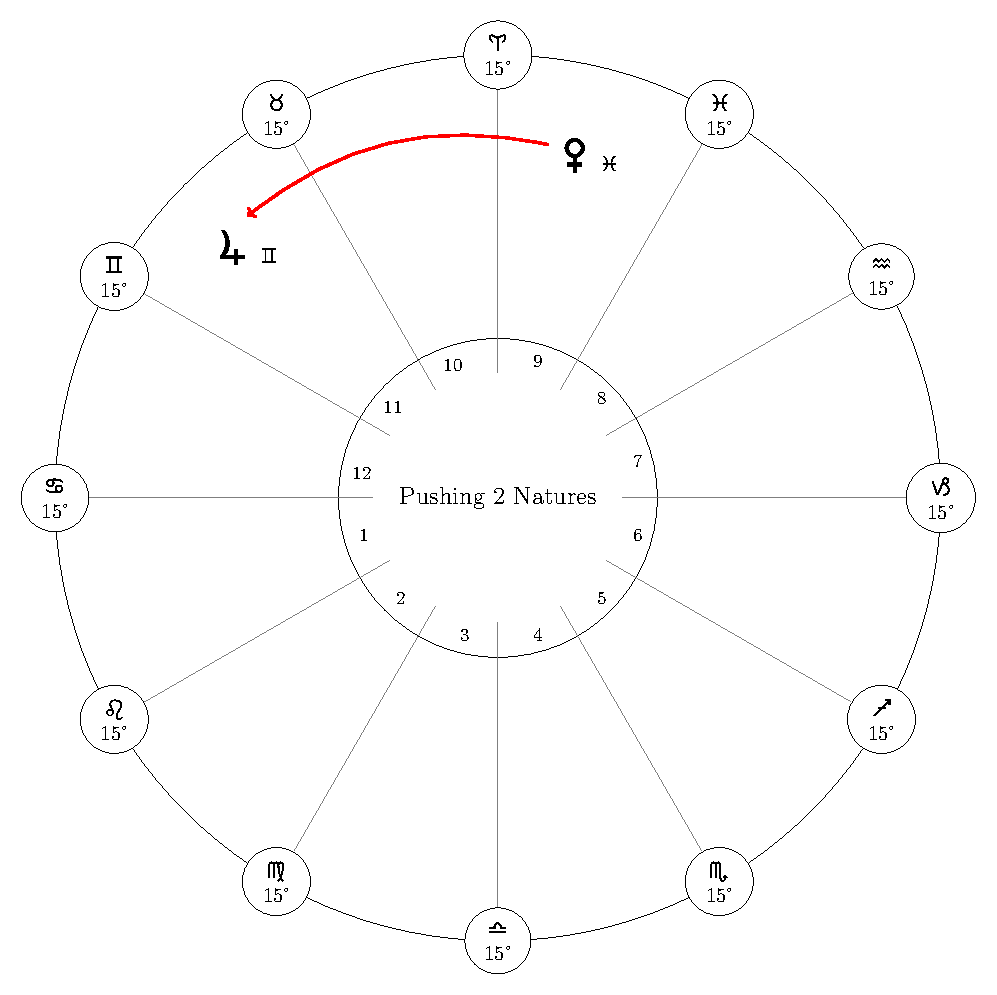
\includegraphics[width=\textwidth]{charts/01-pushing-two-natures}} \\
\end{center}

\end{columns}
\footnotetext[1]{Abu Ma'shar p25; Ibn Ezra p122 calls it \textsl{"conferring of two natures"}}
\end{frame}

% ----------------------------------------------------
\subsubsection{Mutual Reception}
\begin{frame}[t]{What Constitutes Reception - Mutual Reception}
\begin{columns}[T, onlytextwidth]
\column{0.5\textwidth}
\textbf{Example:} \Mars\ 10 \Capricorn\ $\Rightarrow$ \Square\ \Saturn\ 20 \Aries \\
\ul
\vspace{0.25cm}
\Mars\ is in \Saturn's domicile (\Capricorn) applying to \Saturn \\
\Saturn\ is in \Mars's domicile (\Aries), therefore, \\
\Mars\ receives \Saturn\ by domicile, and \\
\Saturn\ receives \Mars\ by domicile \\
\vspace{0.25cm}
giving  \textbf{Mutual Reception} [MR] by \textsl{domicile} \\
so \Mars\ receives \Saturn\ and commits his disposition to him and \Saturn\ receives it\footnotemark[1]\\
\vspace{0.25cm}
This is the strongest form of reception; the second strongest form occurs when there is mutual reception by \textsl{exaltation}. e.g. both planets are in each other's sign of exaltation. i.e. \Venus\ in \Cancer\ \Trine\ \Jupiter\ in \Pisces.

\column{0.5\textwidth}

\begin{center}
{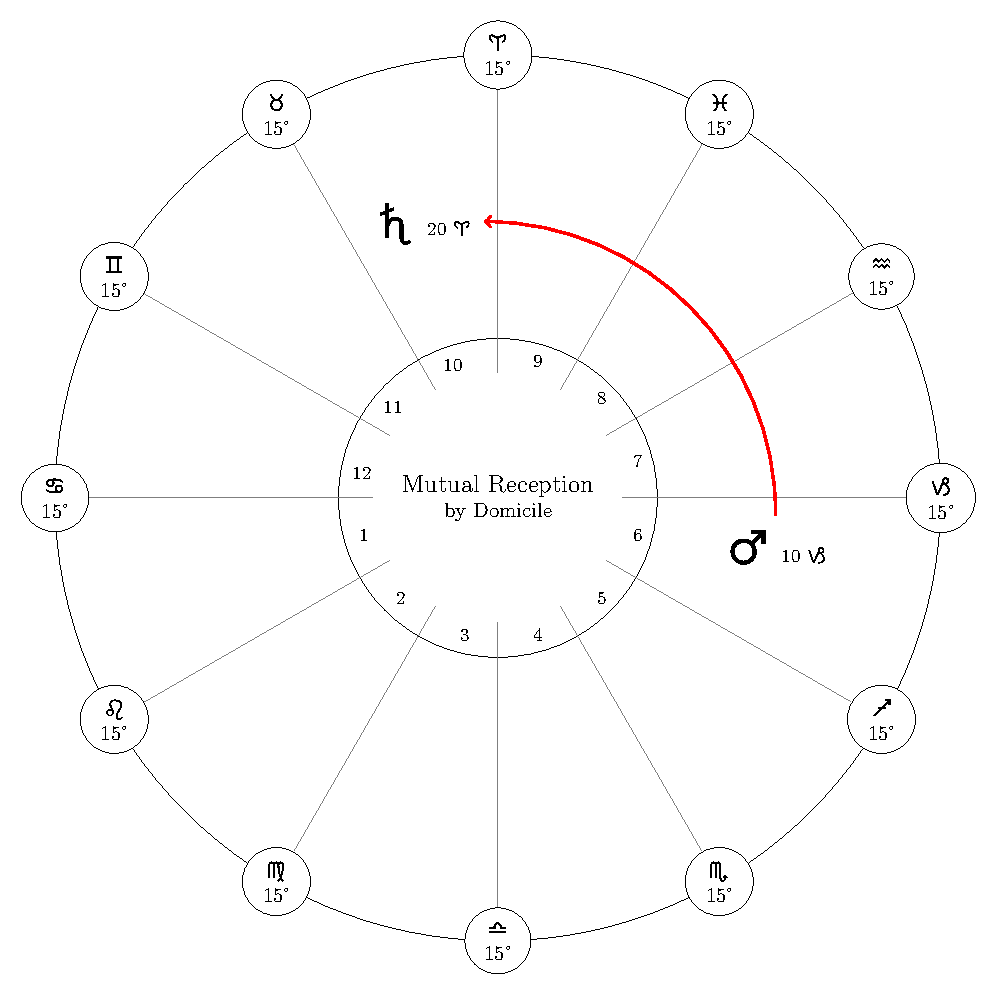
\includegraphics[width=0.9\textwidth]{charts/01-MR-by-domicile}} \\
\end{center}

\end{columns}
\footnotetext[1]{Masha'allah [RH] p3; note that Sahl would call this a non-reception as \Saturn\ is in his Fall.}
\end{frame}
% ---------------------------------------------
\subsubsection{Corrupted Receptions and Returns}
\begin{frame}[t]{What Constitutes Reception - Corrupted Receptions or Returns}
There can be \textbf{no reception} if neither planet has dignity in their own or the other planet's place e.g. \Mercury\ $\Rightarrow$ \Jupiter\ in \Taurus\ where both are peregrine. Although Masha'allah does describe a situation which allows for eventual reception if the applied to planet (\Jupiter\ in this example) goes on to apply, with reception, to a third planet.\\
\vspace{0.25cm}
While Sahl denies reception if a planet is in his own Fall or applying to another planet from that planet's Fall, the other authors appear to accept the reception but say that it is \textbf{corrupted or greatly diminished} i.e. the outcome to the matter is far less than what was hoped for or fails to last.\\
\vspace{0.25cm}
As well, a receiving planet that is \textbf{retrograde} or \textbf{USB} will \textbf{return} what it received, destroying it in the process. The same occurs if both planets are cadent.\footnotemark[1] \\
\vspace{0.25cm}
Still another form of return occurs when a planet applies to a cadent planet, in which case Sahl says the matter \textsl{"will not have an ending"}.

\footnotetext[1]{Sahl [Holden] p20}
\end{frame}
% ----------------------------------------------------
\begin{frame}[t]{What Constitutes Reception Continued}

Masha'allah tells us that if the matter being analyzed has to do with a King, the Exaltation rulers will have more authority over the matter than the domicile rulers.

As a general rule, reception is stronger if the planet applied to (usually the heavier planet) receives the applying planet (usually the lighter planet).

The later authors (Sahl, Abu Ma'shar, Ibn Ezra) also allowed reception by triplicity, term, and face but only considered it to be an \textsl{effective} reception if it involved at least two of these minor dignities i.e. received by triplicity and term or triplicity and face or term and face. Masha'allah does mention these minor dignities in his \textsl{Book of Thoughts and Intentions} but only in relation to determining which planet has the most authority over a specific matter; he does not use them in any of his \textsl{On Reception} examples.\footnotemark[1]
\begin{block}{}
Reception is important as it implies completion; that the matter will be disposed of, effected, by the receiving planet; that what the significator commits to another will be brought into being and realized.
\end{block}
\footnotetext[1]{Although Sahl does claim that Masha'allah allowed reception by the minor dignities [JH p18].}
\end{frame}

\section{Horary Rules}
\subsection{Questions in General}
\begin{frame}[t]{Questions in General}

A question must be of great concern or necessity for the querent (the one asking the question); and they should not ask further questions with regard to the matter until the first question has been understood and examined (i.e. no compound questions).

An astrologer should not look to answer his own questions as \textsl{"it does not suit a wise man to look for himself"}. 

To examine the question, draw up a chart for the time the question is asked or verbally put to the astrologer; or, if in the form of a letter, the moment when the astrologer understands what is asked; calculating the Asc, the MC, the places of the 7 planets, and note who disposits each of them and which houses they are in.
\vspace{0.5cm}
\begin{mdframed}[backgroundcolor=gray!5, rightmargin=2em, leftmargin=2em]
\textbf{Note:} James Holden thinks the calculation of the MC implies a quadrant system of houses, most likely Alchabitius, but he acknowledges that Masha'Allah, in later examples, appears to be using a Sign-House system; most likely Equal House\footnote{In Holden's translation of Masha'Allah's \textsl{The Book of Thoughts} he indicates that either the Alchabitius or Equal House system were used.}
\end{mdframed}

\end{frame}
\subsection{Choosing Significators}
\begin{frame}[t]{Choosing Significators}
Masha'Allah's method for choosing which planets will act as significators for the person asking the question (the \textsl{querent}) and the question's subject matter (the \textsl{quesited}), can be reduced to:
\begin{itemize}
\item Does the ruler of the Ascendant (L1) aspect the 1st House?
	\begin{itemize}
		\item Yes? use L1 as the main significator of the querent and the \Moon\ as their partner
		\item No? does L1 aspect another planet that aspects the 1st House or one who does so indirectly by aspecting a 3rd planet that aspects the 1st House?
			\begin{itemize}
				\item Yes? work through these planets and use the \Moon\ as a their partner
				\item No? repeat the same steps using the \Moon\ instead of L1 and if she is suitable, make her the main significator and L1 her partner
			\end{itemize}
	\end{itemize}
\item If neither L1 nor the \Moon\ are usable, see which of the two is the first to leave its sign and judge the effect from that planet's first joining to another planet after entering its new sign, using the other planet (L1 or \Moon) as their partner;\footnote{Normally the \Moon\ is the first to change signs as she moves faster than the other planets.} noting that matters will be slow and inactive until the sign change occurs.
\end{itemize}

\end{frame}
% ------------------------------------------------------------------------------------------
\begin{frame}[t]{Choosing Significators Continued}
\begin{itemize}
\item The main significator of the matter being asked about will be the ruler of the house signifying the matter i.e. Life, ruler of 1st House (L1); Wealth, ruler of 2nd House (L2); Siblings, ruler of the 3rd House (L3); etc.
\item Planets in the 1st House and the house signifying the matter at hand have a bearing on the conditions surrounding the matter BUT they do not determine the outcome of the matter; that depends on the chosen house rulers, their aspects and condition.\footnote{Robert Hand says \textsl{"Rulers of houses in general are more important to outcomes than occupants of houses."}}
	\begin{itemize}
		\item planets in the affected houses, if they are received by their dispositor, \textsl{"indicate the goodness and worthiness of the thing sought"}, if they are not received by their dispositor, then they indicate impediments and the worthlessness of what is sought
	\end{itemize}
\item If the ruler of the Asc or the \Moon\ does not aspect the 1st House it to be considered \textsl{evil and impeded}
\end{itemize}

\end{frame}
\subsection{Perfection and Outcomes}
\begin{frame}[t]{Perfection and Outcomes}
\begin{block}{}
\textsl{Perfection (the performance of a thing) is perhaps known from the planet to which the ruler of the Asc is first joined; from the \Moon; or from the second one that receives the commitment [of the disposition], or namely from whichever one is the last reception [and] there will be the end; or from the ruler of the thing quesited; or from a benefic that is in a good place without reception.} [JH p36]
\end{block}
\textsl{Perfection} can come about in a number of ways ([RH p31, 34])
\small
\begin{itemize}
\item significator of the querent (A) to the significator of the quesited (B), with or without reception, and \textsl{B} does not commit his disposition to a third planet (C)
\item L1 joining a benefic in the house signifying the matter
\item L1 joining a malefic with dignity in the house signifying the matter
\item L1 joining, and received by, an undignified malefic in the house signifying the matter
\item significator of the quesited to L1, with or without reception, or, to planets in the 1st (under the same conditions described for L1 to planets in the house of the matter signified)
\item L1 or the \Moon\ to an angular or strongly dignified benefic, with or without reception; or, a malefic, similarly placed, with reception
\end{itemize}
\end{frame}
% -----------------------------------------
\begin{frame}[t]{Outcomes Continued}

If \textsl{A} is the significator of the querent and receives \textsl{B}, the significator of what is sought; the querent will get what he has been seeking but if \textsl{A} is the significator of what is sought and \textsl{B} is the significator of the querent, then the querent will get what has been asked about without any seeking of it on his part. [JH 38]

Outcomes are better, stronger, more readily done, and stable, and durable if the significator of the quesited receives the significator of the querent. [JH 38]

\begin{block}{}
\textsl{"Reception will not be destroyed in any way whatsoever,...,if the planet which receives has rulership over a matter, and it is the dispositor [of the querent's significator] and the disposition comes to it [the querent's significator applies to it], and if it does not commit disposition to another. Because if it should commit disposition to another planet after its own reception, the reception signifies the accomplishment of the matter, and the commission of its disposition to another planet signifies the end of the matter and to what [state] its final affairs would come."} [RH p32]
\end{block}
So if A applies to its dispositor B, it is received and the matter is accomplished. If B happens to then apply to another planet C, the conditions of that application indicate how the matter will eventually play out.
\end{frame}
% -----------------------------------------
\begin{frame}[t]{Outcomes Continued}

\begin{block}{}
\textsl{"After that, the ruler of the house of the thing [quesited] is looked at to see to what planet it commits its own disposition after its effecting...if it is a benefic, they say the thing will be made better. And if it is a malefic, they say that the thing will be subsequently destroyed."} [JH]p22
\end{block}
If an application by L1 or the \Moon\ shows that the matter will be completed; look to the ruler of the matter being sought (the ruler of the quesited) to see how the matter will play out once it has been effected.

The exception is if the question is about death as there is nothing that can come after it.

If the first joining of the querent's significator is to a malefic and does not involve reception and if the malefic is not the significator of the quesited;  a \textbf{prohibition} is indicated [JH p35].

\end{frame}
\subsection{1-3 Perfection, Deterioration, and Connection}
\begin{frame}[t]{Sahl's Modes: 1-3 Perfection, Deterioration, and Connection}
Sahl summarizes the ways in which a matter can be perfected or destroyed as follows:\footnotemark[1]

\begin{description}[style=nextline]
\item[1. Perfection or Advance] (\textsl{alichel}) when a planet is in an angular or succedent house (Ibn Ezra says "it indicates a favourable result").

\item[2. Deterioration or Retreat] (\textsl{alicher}) when a planet is cadent (Ibn Ezra says "the person will give up the matter")

\item[3. Conjunction or Connection] (\textsl{alittisal}) if A is applying to \Conjunction\ B, they are connected until they are separated by 1°, or, if A \Conjunction\ B in the same sign, they are connected until A moves past B (the heavier planet) and B is no longer within A's light (1/2 its orb) \\
\vspace{1em}
\textsl{"Whenever one planet aspects another and within its own light strikes the degree of that other, it is said to be conjoined to it; and if it does not strike it within its own light, it is not said to be conjoined but rather "going to conjunction."} [JH p14]\\

\end{description}

\footnotetext[1]{[JH] p12-25. Bonatti, in his \textsl{Considerations} \#4, gives a similar list.}
\end{frame}
% ---------------------------------------
\subsection{4-5 Separation, Translation}
\begin{frame}[t]{Sahl's Modes: 4-5 Separation, Translation}
\begin{description}[style=nextline]
\item[3. Connection Cont'd] A planet at the end of a sign, not joined to another, but striking a planet in the next sign with its light or being within the other planet's light, is conjoined to it even though it is blind (averse) to it\footnotemark[1]. e.g. \Moon\ 27 \Aries\ is conjoined to \Venus\ 2 \Taurus. They "perfect after despair" if they join in the next sign before another connects to either of them (Ibn Ezra p131). \\
\vspace{1em}
\textbf{Planet's Light Before and Behind:} \Sun: 15°; \Moon: 12°; \Venus\ \& \Mercury: 7°; \Jupiter\ \& \Saturn: 9°; \Mars: 8°. \\

\item[4. Separation] (\textsl{alitiuctraf}) separation occurs when one planet overtakes and passes another either by conjunction or aspect but \textsl{"an aspect is from one sign to another, while a conjunction is said to be from one degree to another"}. \\

\item[5. Translation] \textsl{(anualac)} translation of light occurs when a planet A is separating from a planet B and immediately applies to a third planet C; A is said to \textsl{carry the nature} of B to C. 
\end{description}

\footnotetext[1]{This could be an argument for out-of-sign conjunctions, especially given what is said under \textsl{Separation}.}
\end{frame}
% -------------------------------------------------------
\begin{frame}[t]{Translation of Light  - A Question of Marriage}
\begin{columns}[T, onlytextwidth]
\column{0.5\textwidth}
\Mercury\ (L1) (querent) \Quincunx\ \Jupiter\ (L7) (marriage) \\
\Moon\ separating \Sextile\ \Mercury\ applying \Square\ \Jupiter \\
\vspace{0.25cm}
Therefore, the \Moon\ was carrying the light of \Mercury\ to \Jupiter\ \textsl{"and this signified the completion of the thing, i.e. the attainment of the woman through the hands of go-betweens and those running back and forth between the two [parties]."} ([JH] p14-15) \\
\vspace{0.15cm}
\textbf{Note:} \\
\small
In this example, it would seem that the \Moon\ is really the querent's significator as \Mercury\ does not aspect the 1st house nor does he aspect \Jupiter. \\

Looking at the \Moon\ \Sextile\ \Mercury\, could the \Mercury\ reception be of a 'pushing nature' variety? with \Mercury\ doing the pushing rather than the applying \Moon\, who does not receive \Mercury?\footnotemark[1]

\column{0.5\textwidth}
\begin{center}
{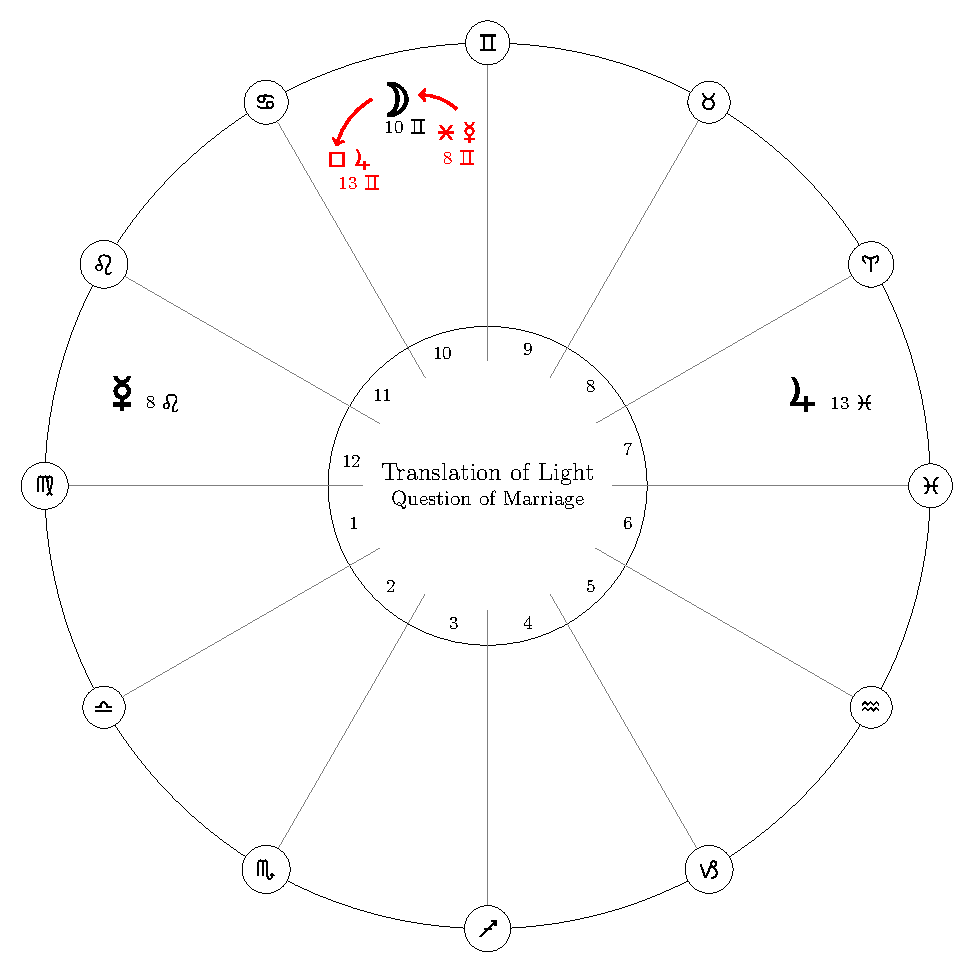
\includegraphics[width=0.9\textwidth]{charts/60-translation}} \\
\end{center}
\end{columns}
\footnotetext[1]{Ibn Ezra "conferring of nature" p121}
\end{frame}
% -------------------------------------------------------
\subsection{6. Conjunction (Collection) of Light}
\begin{frame}[t]{Sahl's Modes: 6. Conjunction (Collection) of LIght}
\begin{description}[style=nextline]
\item[6. Collection of Light] (\textsl{algemee}) when 2 planets, not in aspect themselves, both connect to a 3rd, heavier planet, that planet is said to collect their light
\vspace{0.25cm}
\begin{columns}[T, onlytextwidth]
\column{0.5\textwidth}
\textbf{Example:} A question about whether a king would acquire a kingdom \\
\ul
\Venus\ (L1) and \Moon\ (L10) are averse (\Semisextile) \\
\Jupiter\ is in the 10th, the house of the kingdom \\
both \Venus\ and the \Moon\ are joined to \Jupiter \\
\vspace{0.25cm}
\textsl{"This signified the acquisition of the kingdom through the hands of some judge or bishop or the hands of some chosen man to whom both planets freely gave their assent."} (p15). \\
\vspace{0.25cm}

\column{0.5\textwidth}
\vspace{-0.5cm}
\begin{center}
{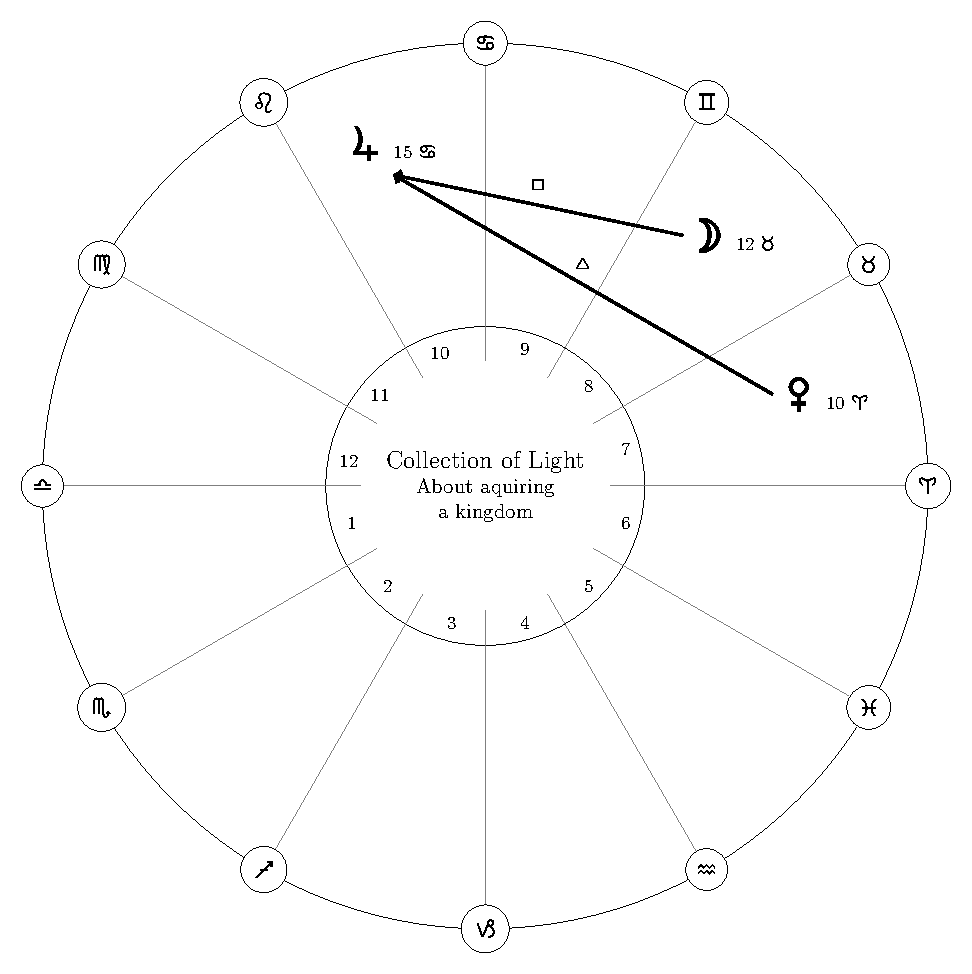
\includegraphics[width=0.9\textwidth]{charts/61-collection}} \\
\end{center}
\end{columns}
\end{description}
\end{frame}
% ------------------------------------------------
\subsection{7 Prohibition}
\begin{frame}[t]{Sahl's Modes: 7 Prohibition ("cutting", "intervention", "nullification")}
Prohibition (\textsl{almane}) is found in 3 modes:\footnotemark[1]  \\
\begin{columns}[T, onlytextwidth]
\column{0.5\textwidth}
\vspace{0.25cm}
\textbf{(i) Abscission ("cutting") of Light} \\
occurs when the significators are conjoining but between them is a 3rd planet who the 1st significator conjoins before it can connect with the 2nd significator. \\

\vspace{0.25cm}
\textbf{Example:} a question of marriage \\
\ul
\Mercury\ (L1) conjoins \Square\ \Mars\ before it conjoins \Trine\ \Jupiter (L7) \\
so \Mars's cuts off \Mercury's light from \Jupiter, prohibiting the marriage. \\

\vspace{0.15cm}
And Sahl says \textsl{"the destruction of this thing would be from the description of the dowry"} as \Mars\ is in the 8th house (the bride-to-be's property).

	
\column{0.5\textwidth}
\vspace{-0.5cm}
\begin{center}
{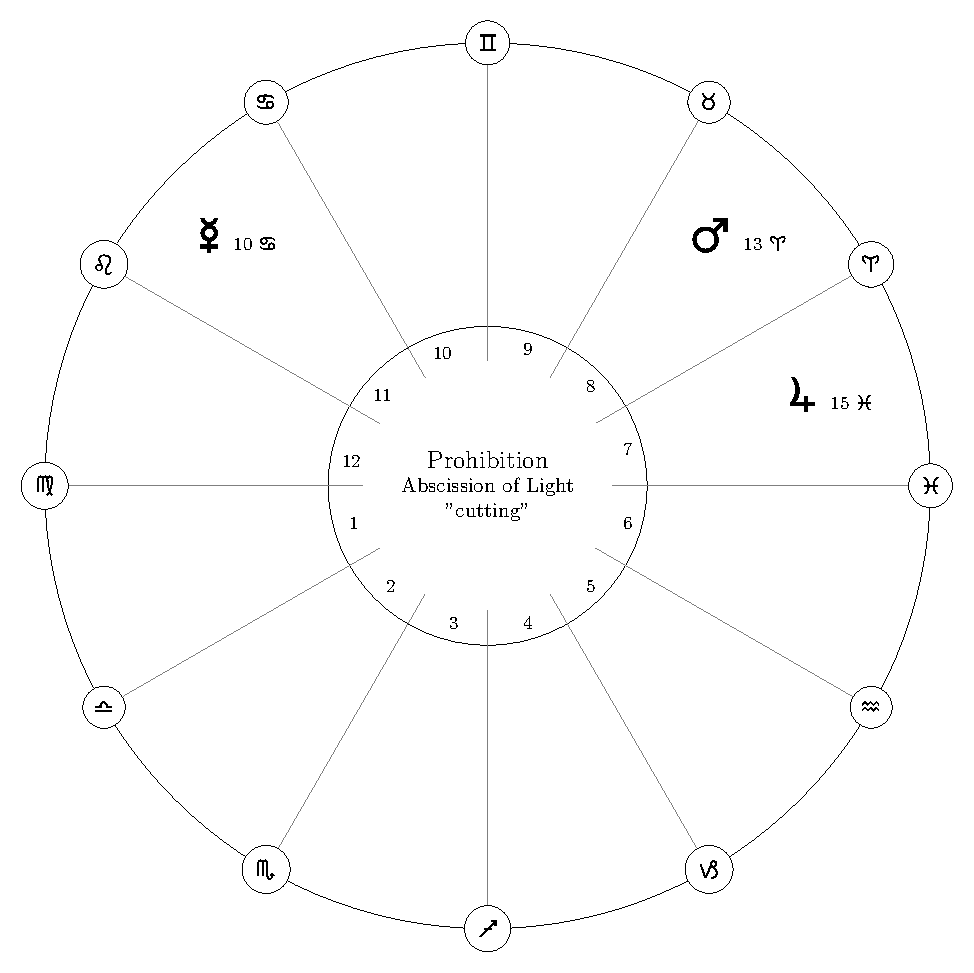
\includegraphics[width=0.9\textwidth]{charts/62-abscission}} \\
\end{center}
\end{columns}
\footnotetext[2]{Dykes calls the 3 modes  "cutting", "intervention", and "nullification" (p56-7)}
\end{frame}
% --------------------------------------------------
\begin{frame}[t]{Sahl's Modes: 7. Prohibition: "intervention"}
\begin{columns}[T, onlytextwidth]
\column{0.5\textwidth}
\vspace{0.5cm}
\textbf{(ii) "intervention"} occurs when 2 significators are in the same sign and a 3rd planet, between them, conjuncts the heavier, 2nd significator  \\

\vspace{0.25cm}
\textbf{Example:} a question of marriage \\
\ul
\Moon\ is L1 and significator of the querent \\
\Saturn\ is L7 and significator of the marriage \\

\vspace{0.25cm}
\Mars\ is between the \Moon\ and \Saturn\ and already conjoined with \Saturn\ (being only 2° from it), effectively intervening between the \Moon\ and \Saturn\ and so prohibiting the  marriage
	
\column{0.5\textwidth}
\begin{center}
{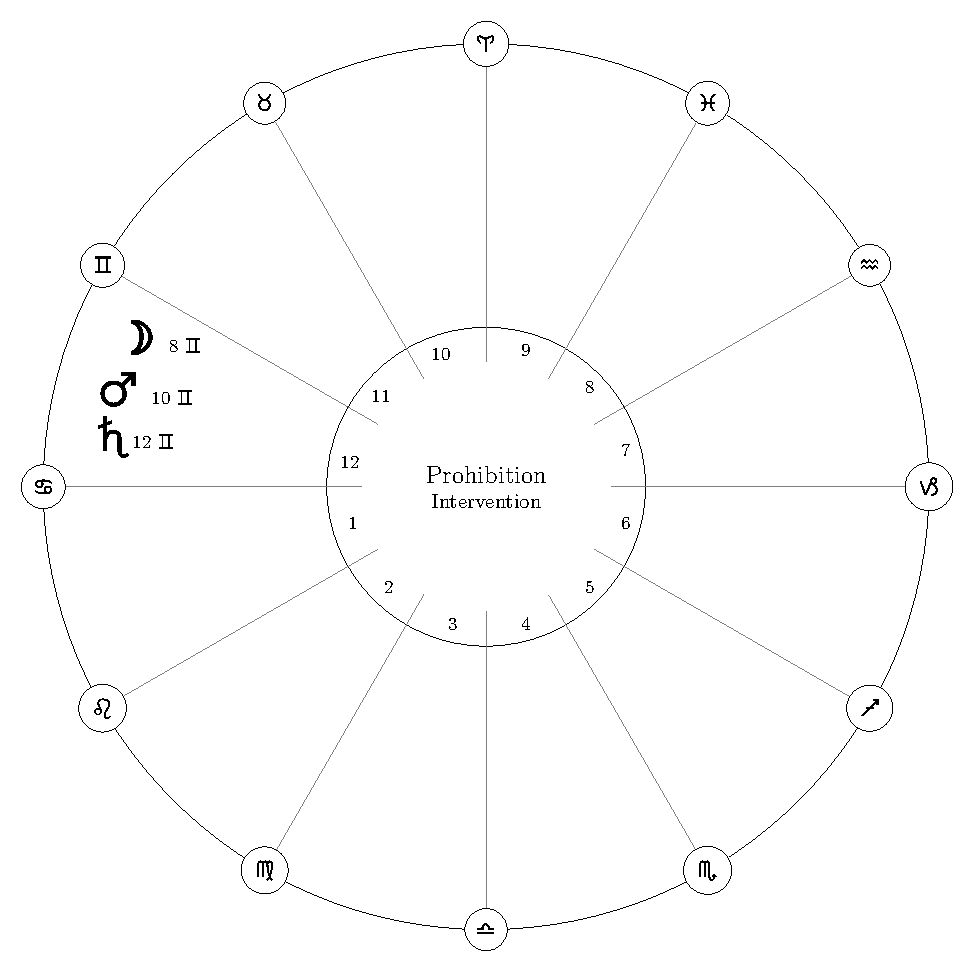
\includegraphics[width=0.9\textwidth]{charts/63-intervention}} \\
\end{center}
\end{columns}
\end{frame}
% -------------------------------------------------
\begin{frame}[t]{Sahl's Modes: 7. Prohibition: "nullification"}
\begin{columns}[T, onlytextwidth]
\small
\column{0.5\textwidth}
\vspace{0.5cm}
\textbf{(iii) "nullification"} when 2 significators are in the same sign and a 3rd, lighter planet, passes the 1st significator to complete an aspect to the 2nd significator, that joining is nullified by the conjunction as \textsl{"an aspect does not destroy a conjunction, but a conjunction does destroy an aspect"} [JH p16-17]

\vspace{0.25cm}
\textbf{Example:} a question of marriage \\
\ul
\Moon\ is L1 and significator of the querent \\
\Saturn\ is L7 and signifcator of the marriage \\ [1em]

\Mars\ is seen to be \Conjunction\ \Saturn \footnote{Planets in the same sign are considered conjunct if they are within 15° of each other.} and so \textsl{"consequently it was cutting off the aspect between the \Moon\ and \Saturn"}, prohibiting their joining and hence the marriage.\\
\vspace{0.25cm}

\column{0.5\textwidth}
\begin{center}
{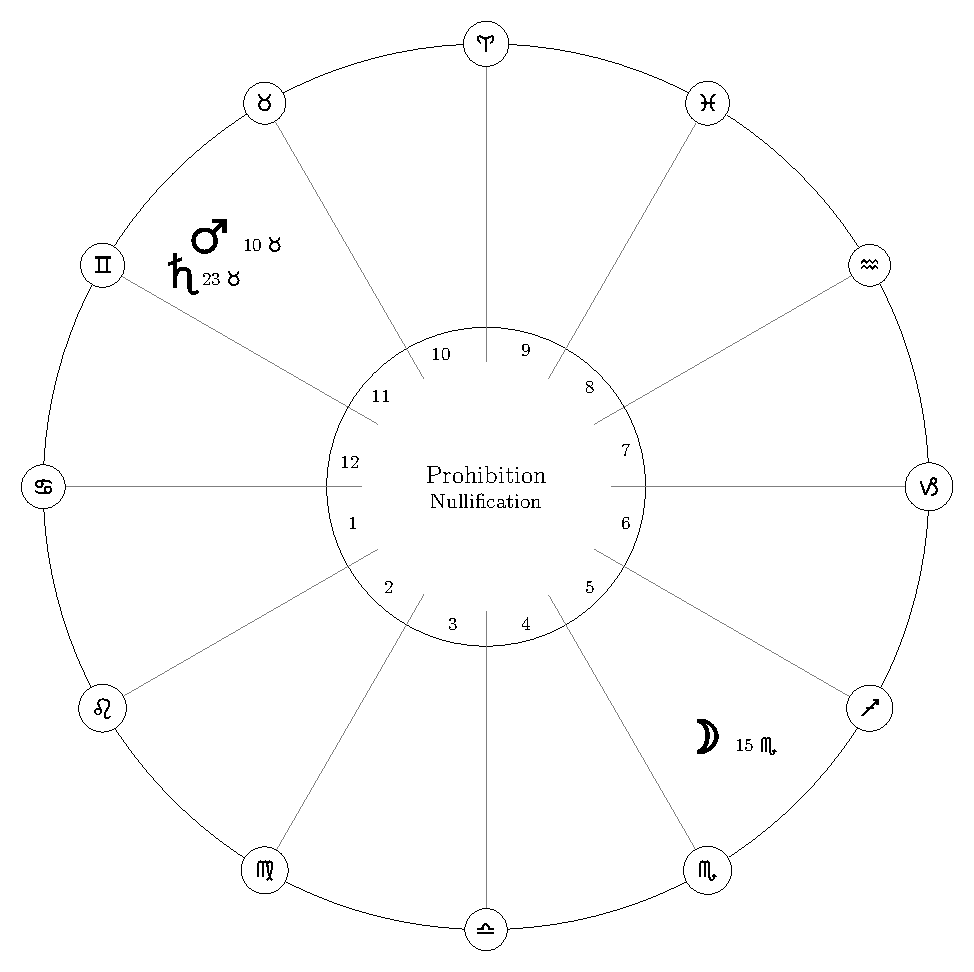
\includegraphics[width=0.9\textwidth]{charts/64-nullification}} \\
\end{center}
\end{columns}
\end{frame}
% ------------------------------------------------------
\begin{frame}[t]{Sahl's Modes: 7. Prohibition: "nullification" cont'd}
\begin{columns}[T, onlytextwidth]
\column{0.5\textwidth}
\footnotesize
Another example, when two planets are joined in one sign (\Moon\ and \Mars\ here) and the lighter planet (\Moon) joins a third planet (\Venus) by aspect and commits its disposition before it completes its \Conjunction\, the judgment is from the planet that is in the same sign because \textsl{"conjunction of this sort is, as we have said, stronger than an aspect."} \\
\vspace{0.1cm}
Sahl also says \textsl{"And when one planet is joined to another, but before it comes to it, it is joined to a third; and when it has been joined to that one, the conjunction itself is destroyed"} [JH 17]

\vspace{0.25cm}
I think he's speaking of 3 planets (A B C) together with A joined to both B and C, in this case A connects to B first and B handles the matter; A's joining with C is broken.\footnotemark[1] 

\column{0.5\textwidth}
\begin{center}
{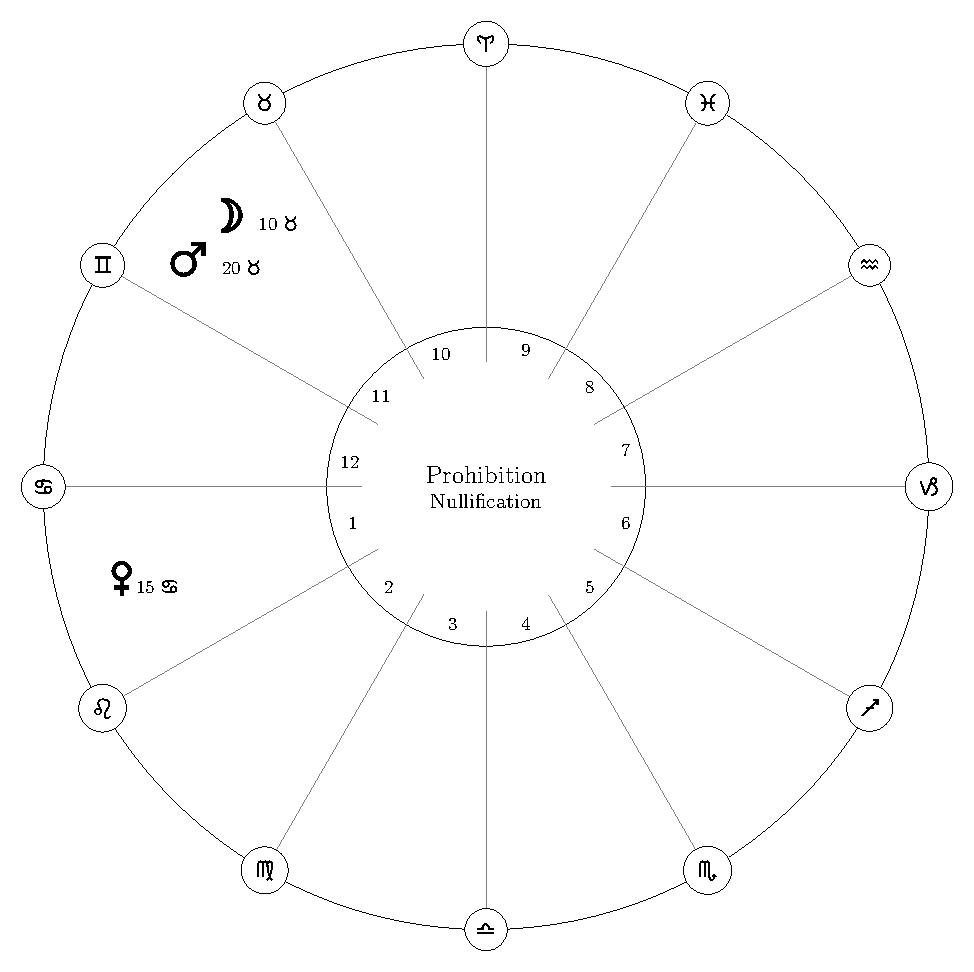
\includegraphics[width=0.9\textwidth]{charts/64a-nullification}} \\
\end{center}
\end{columns}
\footnotetext[1]{Unfortunately Dykes text doesn't have this sentence so no way to double check my reading; however, Ibn Ezra describes the same under his definition of Prohibition (p.122)}
\end{frame}
% --------------------------------------------
\subsection{8 Reception}
\begin{frame}[t]{Sahl's Modes: 8. Reception}
\small
\begin{columns}[T, onlytextwidth]
\column{0.5\textwidth}
\textsl{(alchobol)} Reception occurs when a planet joins another from that planet's domicile or exaltation (perfect reception) or from two of the other planet's minor dignities (triplicity, term, face). \\

\vspace{0.25cm}
\textbf{Example:} \\
\ul
\Moon\ in \Aries\ in \Trine\ to \Mars\ in \Sagittarius \\

\vspace{0.25cm}
\Mars\ will receive the \Moon\ because she occupies his (\Mars) domicile. Similarly, if she was joined to the \Sun, as \Aries\ is his exaltation; or if she was in \Taurus\ and joined to \Venus, or in \Gemini\ and joined to \Mercury; in each case she would be received as she would occupy the domicile or exaltation of the planet she was conjoining. \\

\vspace{0.25cm}
And if the \Moon\ was void of course but on moving into the next sign she was joined to the domicile or exaltation ruler of the first sign, she will be received but if she first joins another planet in her new sign, she will be impeded [JH p19]


\column{0.5\textwidth}
\begin{center}
{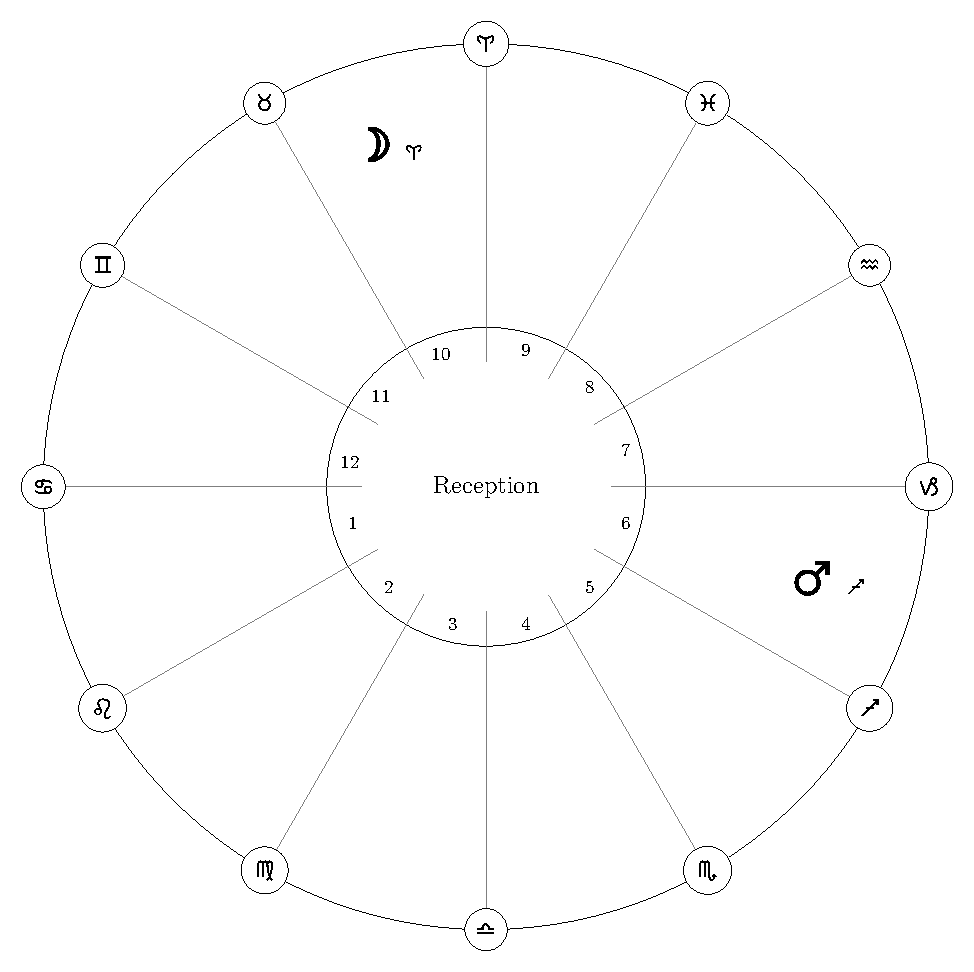
\includegraphics[width=0.9\textwidth]{charts/65-reception}} \\
\end{center}
\end{columns}
\end{frame}
% ---------------------------------
\subsection{9 Not Received}
\begin{frame}[t]{Sahl's Modes: 9. Not Received}
\footnotesize
\begin{columns}[T, onlytextwidth]
\column{0.5\textwidth}
\textsl{(gattalchobol)} There can be no reception between two planets (A $\Rightarrow$ B) if: \\
\vspace{0.25cm}
(i) A is in the sign of B's Fall (\Moon\ \Square\ \Saturn) \\
(ii) A is in its Fall and B is peregrine there (\Venus\ \Sextile\ \Jupiter) \\
(iii) B is peregrine in the sign A occupies (\Jupiter\ \Trine\ \Saturn)\\
(iv) B is in the sign of A's Fall (\Mercury\ \Square\ \Mars) \\
(v) B is in the sign of its own Fall \\
\hspace{1em}i.e. \Moon\ in \Gemini\ \Trine\ \Sun\ in \Libra\ (not shown) \\
\vspace{0.25cm}
According to Sahl, a planet with no \textsl{testimony} (dignity) in a place cannot recognize the planet that is applying to it and so cannot receive it. \\

And he says A in B's fall \textsl{"will be like someone who comes to him [B] from the house of his enemies--it does not receive it nor esteem it."} (i) \\

And a planet in its own Fall conjoined to a planet with no dignity in that same sign will see the other planet \textsl{"for nothing, as if an unknown garment should be given to anyone asking"}. (ii)\\

And a planet joined to another in its own Fall \textsl{"makes him descend, and it diminishes what will come to him"}. (v)

\column{0.5\textwidth}
\begin{center}
{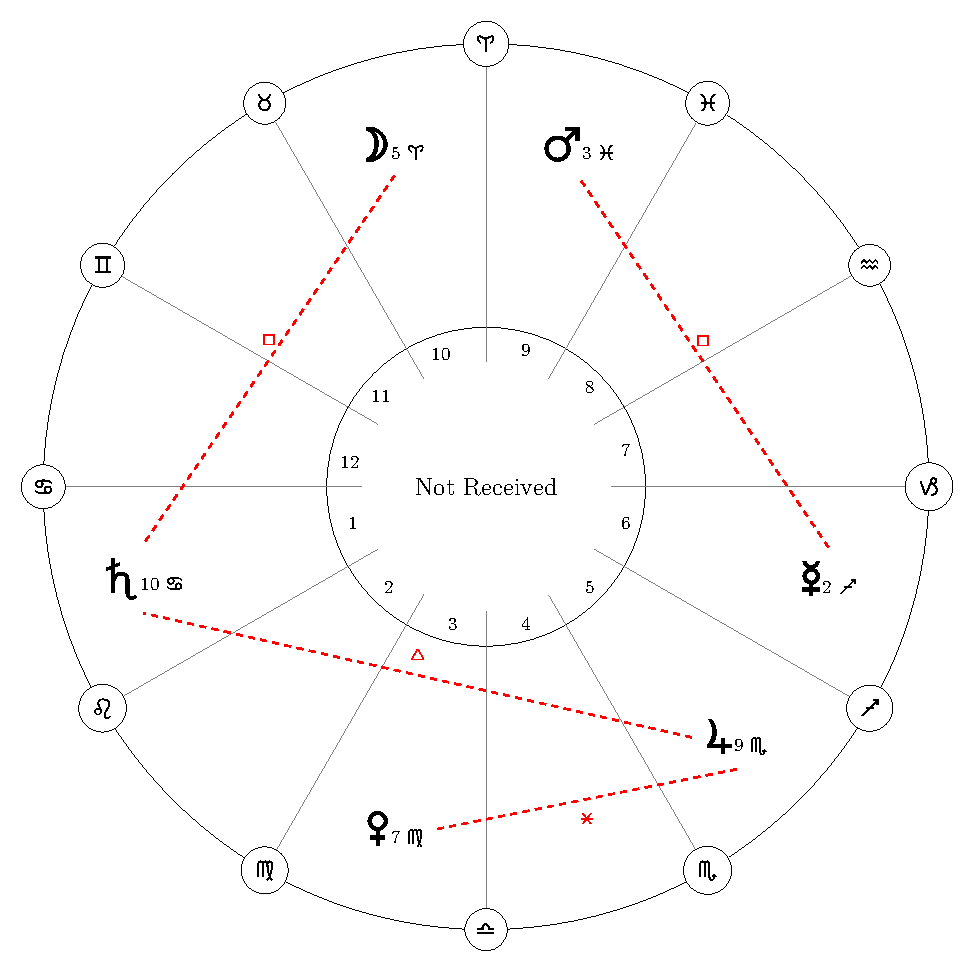
\includegraphics[width=0.9\textwidth]{charts/66-not-received}} \\
\end{center}
\end{columns}
\end{frame}
% ---------------------------------------
\subsection{10-13 Void of Course (VOC), Return, Giving Virtue}
\begin{frame}[t]{Sahl's Modes: 10-13 Void of Course (VOC), Return}
\begin{description}[style=nextline]
\item[10. Void of Course] \textsl{(halaaceir)} void of course occurs when a planet is separating from one planet and not joined to (in the light of) any other planet before it leaves the sign it is in. (A \textbf{feral} planet forms no aspect, separating or applying, in the sign it occupies.)

\item[11. Return] \textsl{(atrad)} Return occurs when a planet is retrograde or USB. In such situations the planet will return whatever it receives, destroying the matter. The same also occurs if both planets are cadent i.e. \Moon\ in the 6th applying to \Mars\ in the 12th which \textsl{"denotes destruction of the beginning of the question and [also] its end."} And if A is angular and only B is cadent, it signifies the beginning of a matter that will not have an end.

\item[12-13. Giving Virtue and Nature] \textsl{(defaalchota)} a planet in its own domicile or exaltation is joined to another planet i.e. \Moon\ in \Cancer\ or \Taurus\ joined to \Jupiter\ or any other planet \textsl{"gives its virtue"} (nature) and commits its disposition. When she is not in \Taurus\ or \Cancer\ she just gives her dispostion.\footnotemark[1]
\end{description}
\footnotetext[1]{Here I think \textsl{disposition} refers to a planet's significations while \textsl{virtue} refers to its authority and power.}
\end{frame}
% ------------------------------------------------
\subsection{14 Strength of the Planets}
\begin{frame}[t]{Sahl's Modes: 14. Strength of the Planets [to Realize Events]}
\textsl{(alchoe)} There are 11 modes in which a planet can effectively execute the disposition of another planet, these occur when the planet is:
\begin{enumerate}
\item[1.] in a good place i.e. angular or succedent
\item[2.] in its own dignities i.e. domicile, exaltation, or in 2 minor dignities
\item[3.] direct in motion
\item[4.] not joined to a malefic by conjunction, square, or opposition
\item[5.] not in its Fall or joined to a planet in Fall or in a cadent place
\item[6.] received
\item[7.] superior (\Mars, \Jupiter, \Saturn) and oriental of the \Sun\ or inferior (\Mercury, \Venus) and occidental of the \Sun
\item[8.] \textsl{"in their own light"} i.e. a diurnal planet above the horizon in a day chart, a nocturnal planet above the horizon in a night chart
\item[9.] in a fixed sign (\Taurus, \Leo, \Scorpio, \Aquarius)
\end{enumerate}
\end{frame}
% -------------------------------------------------------------------
\begin{frame}[t]{Sahl's Modes: 14. Strength of the Planets Continued}
\begin{enumerate}
\item[10.] in the "heart of the \Sun" which happens when it is in the same degree as the \Sun\footnotemark[1] \textsl{"because then the fortunes increase good fortune and their good, but the malefics both increase and greatly strengthen their evil"}

\item[11.] a masculine planet in masculine quarters (Asc to MC, Desc to IC) and signs or a feminine planet in feminine quarters (MC to Desc, IC to Asc) or signs
\end{enumerate}
\textsl{"These are the testimonies by which the planets are greatly strengthened...for completing the matter when they have received and allowed."} [JH p23] \\ 
or, \\
\textsl{"These are the testimonies which, [when] the planets are in them, they are strong,...when they accept [the management] and make a promise."} [Dykes p67]


\footnotetext[1]{This is usually called \textsl{cazimi} and many authors limit it to a planet within 17' of the \Sun.}
\end{frame}
% --------------------------------------------------------------
\subsection{15 The Debility of the Planets}
\begin{frame}[t]{Sahl's Modes: 15. The Debility of the Planets}
\small
\vspace{-0.2cm}
\textsl{(adoef)} There are 10 modes in which a planet can be debilitated and impeded in a nativity or horary chart; these occur when a planet is:
\vspace{-0.25cm}
\begin{enumerate}
\item[1.] cadent and so not in aspect to the ascending place i.e. in the 6th or 12th place
\item[2.] retrograde
\item[3.] USB i.e. within 17° of the \Sun
\item[4.] \Conjunction, \Square, or \Opposition\ a malefic
\item[5.] besieged by malefics
\item[6.] in its own fall or joined to a planet in its fall
\item[7.] joined to a cadent planet or separating from a planet that was receiving it
\item[8.] peregrine and \textsl{"being pursued by the \Sun, i.e. when it is before the \Sun"}\footnotemark[1]
\item[9.] on the ecliptic (0° latitude) and with the \NorthNode\ or \SouthNode
\item[10.] in its detriment (opposite its domicile) 
\end{enumerate}
\vspace{-0.2cm}
\footnotesize
\textsl{"Follow these modes...with regard to the planet that receives the disposition and the one that promises the matter."} [JH p24]


\footnotetext[1]{Dykes says this means the planet has set before the \Sun\ and is invisible. [p68]}
\end{frame}
% -----------------------------------------------------
\subsection{16 The Defects of the Moon}
\begin{frame}[t]{Sahl's Modes: 16. The Defects of the Moon}
\textsl{(alchamar)} There are 10 ways the \Moon\ can come to be in a bad condition and so detrimental in all questions and initiatives; they are when she is:
\begin{enumerate}
\item[1.] combust i.e within 12° of the \Sun
\item[2.] in her fall (\Capricorn) or joined to a planet in its own fall
\item[3.] within 12° of an exact \Opposition\ with the \Sun
\item[4.] joined to a malefic by \Conjunction, \Square, or \Opposition\ or beseiged by malefics
\item[5.] within 12° of the \NorthNode\ or \SouthNode\ and in the same sign with them
\item[6.] in \Gemini\ (the 12th sign from her domicile) or in the last, and so malefic term, of any sign
\item[7.] cadent or joined to a cadent planet
\item[8.] in the \textsl{Via Combusta}  (19 \Libra\ to 3 \Scorpio)
\item[9.] feral or void of course i.e. not joined to any other planet
\item[10.] slow (moving at less than her average motion) or waning and at the end of the lunar month
\end{enumerate}
\end{frame}
% -------------------------------------------------------------
\begin{frame}[t]{Sahl's Modes: 16. The Defects of the Moon Continued}
\textsl{"These are the...defects of the Moon and its impediments during which no work should be begun,...; and it is not praiseworthy in a nativity [either], or in travel."} [JH p25] \\ \vspace{0.25cm}
\Mars\ harms the \Moon\ most by \Conjunction, \Square, or \Opposition\ when she is waxing as then they are both hot; \Saturn, similarly joined, does not impede her then because he is cold. And in nocturnal charts, when the \Moon\ is waning, and \Mars\ is in a feminine sign, he impedes less but in a day chart, when the \Moon\ is waxing and he is in a masculine sign, he impedes more.

\Saturn\ harms the \Moon\ most by \Conjunction, \Square, or \Opposition\ when she is waning as then they are both cold; \Mars, similarly joined, does not impede her then because he is hot. And in diurnal charts, when the \Moon\ is waxing, and \Saturn\ is in masculine signs, he impedes less but in a nocturnal chart, when the \Moon\ is waning and he is in feminine signs, he impedes more.

\textbf{Impeded:} no planet or sign is impeded unless it is in the \Conjunction, \Square, or \Opposition\ of a malefic.

\textbf{Fortunate:} no planet, or the Asc, is fortunate unless \Venus\ or \Jupiter\ are in its angles.

\end{frame}
% -----------------------------------------------------------------
\begin{frame}[t]{Some of Ibn Ezra's Descriptions of Planet Conditions (Ch.8)}
\footnotesize
\begin{itemize}
\item Any matter will be accomplished according to the strength of the receiving planet
\item A planet is not "declared harmed" unless it is in the light of a malefic
\item A planet separating from aspect of a malefic by at least 1° "will cause fear which is not realized"
\item A benefic aspecting L1, if L1 does not aspect the rising sign, nothing will come to pass
\item Benefics cadent or in signs of opposite nature, detriment, or fall "do not bring benefit at all"; malefics in similar state do little harm
\item Malefics "in great power"  indicate good "except it comes with effort and suffering"
\item \Jupiter\ removes \Saturn's harm (\Venus\ needs \Jupiter's help to do so);  \Venus\ removes \Mars\ harm more so than \Jupiter\ can
\item A planet in Fall "indicates worry, distress, and hardship"
\item A retrograde planet "indicates antagonism, and the destruction of anything that is contemplated"
\item A planet Stationary Direct (SD) about to turn retrograde "is like a person who does not know what to do and the result is unfavourable"; it indicates "difficulty and loss"
\item A planet Stationary Retrograde (SR) about to turn direct "is like a person hoping for something and not losing one's hope"
\end{itemize}
\end{frame}

\subsection{Timing}
\begin{frame}[t]{Timing  [JH 32-33] [RH 27-29]}
When the joining is by aspect (not conjunction) the number of degrees needed to perfect the aspect gives the number of days.

If it doesn't happen then, it will happen when the two join bodily (by a conjunction) in a strong place, an angle or a place where the significator of the matter rejoices.

If not then, it will happen when the planet handling the disposition is rising from the \Sun, renewing itself.

If the significators started off Void of Course, needing to enter a new sign before joining with  another planet, then things will go slowly and matters will be prolonged [JH 17, RH 8]

Angles strengthen, hurry, and fortify the matter, for good or ill, and whatever is signified by the ruler of the disposition, it will last [JH p36] while cadent houses cause delays, little advancement, and only small things [JH p48].

Swiftness of completion, as indicated by the houses; the quickest to the slowest are: \\
Asc, MC, 11th, 7th, 4th, 9th, 5th, 3rd,  with all these being \textsl{"good and praiseworthy"} while the averse houses (8th, 6th, 12th, 2nd) are slowest and "inimical" to the querent [JH p48, RH p46]

\end{frame}

\section{Masha'allah's Example Charts}
\subsection{About Life or Death}
\begin{frame}[t]{About Life or Death [JH p18-19,23,27] [RH p10-11,15,19]}
If a person asks whether he will die during the year, look for indications that:\footnote{If L1 is impeded, use the \Moon\ in its place.}
\vspace{0.25cm}
\begin{columns}[T, onlytextwidth]
\column{0.5\textwidth}
\textbf{They will escape death:}\\
\begin{itemize}
\item L1 to a benefic who is not L8 and who does not pass on disposition or return it to another 
\vspace{0.25cm}

\item L1 to a planet that receives him, and if they are ill, they will recover from their illness
\vspace{0.25cm}

\item \Moon\ joined to L8 but L1 strong and unimpeded
\item L8 joined to and received by L1 \textsl{"will not completely destroy"} life
\end{itemize}

\column{0.01\textwidth}
\rule{.1mm}{.45\textheight}

\column{0.5\textwidth}
\textbf{Death wins out:}\\
\begin{itemize}
\item L1 joined to L8 or vice versa (do not consider the \Moon) 
\item L1 joined to a malefic or L8 without reception and the \Moon\ evil and impeded
\item L1 joined to a malefic in the 8th
\item L1 joined, without reception, to a benefic in the 8th who has dignity there
\item L8 joined to a planet in the 1st
\end{itemize}
\end{columns}
\vspace{0.25cm}
To know if the person will fully recover their  'good fortune and health' examine the planet that signifies escape from death; if it aspects the significator's original position in the chart the person will escape all harm.\footnote{Robert Hand fnp11}
\end{frame}
% -----------------------------------------------------------
\begin{frame}[t]{About Life or Death Continued [JH 27-29][RH 19-22]}
\begin{itemize}
\item when L8 joins and is received by L1, L8 cannot completely destroy life but we need to look at L1 and the \Moon\ and if one signifies life and the other death, the significations of L1 are stronger as it has more significance in the matter of Life than the \Moon; however, as they are partners, the \Moon\ will impact the effects of L1 according to the strength or weakness of L1 and the \Moon

\item L8 is inimical to L1 UNLESS they are the same planet as \textsl{"then it will not impedite itself, even if it is also a malefic"} (and the same is true of L1 and L6)
\end{itemize}

\end{frame}
\subsection{Sickness}
\begin{frame}[t]{Sickness [JH]p19-21, [RH]p11-13 }
The question was about a sick person, \textsl{"whether he would be freed from his sickness, or whether he would die"} \\
\vspace{0.25cm}
\begin{columns}[T, onlytextwidth]
\column{0.5\textwidth}
\Mercury\ (L1)  Void of Course in the 8th signifies \textsl{"the strength of pain and the fear of death"} as does \Mars\ (L8) in the 10th aspecting the 1st who signifies \textsl{"the strength of pain and the loss of hope". } \\

\vspace{0.2cm}
\Mercury (L1) is Void of Course, does not aspect the 1st, and is not first to leave his sign. \\

\vspace{0.2cm}
The \Moon\ is also Void of Course but she is \Trine\ the 1st House and she is the first to enter a new sign so she is the stronger significator. \\

\vspace{0.2cm}
The two significators of the querent, both VOC, signified \textsl{"a prolongation of the sickness"} and its severity.\\


\column{0.5\textwidth}
\begin{center}
\vspace{-0.75cm}
{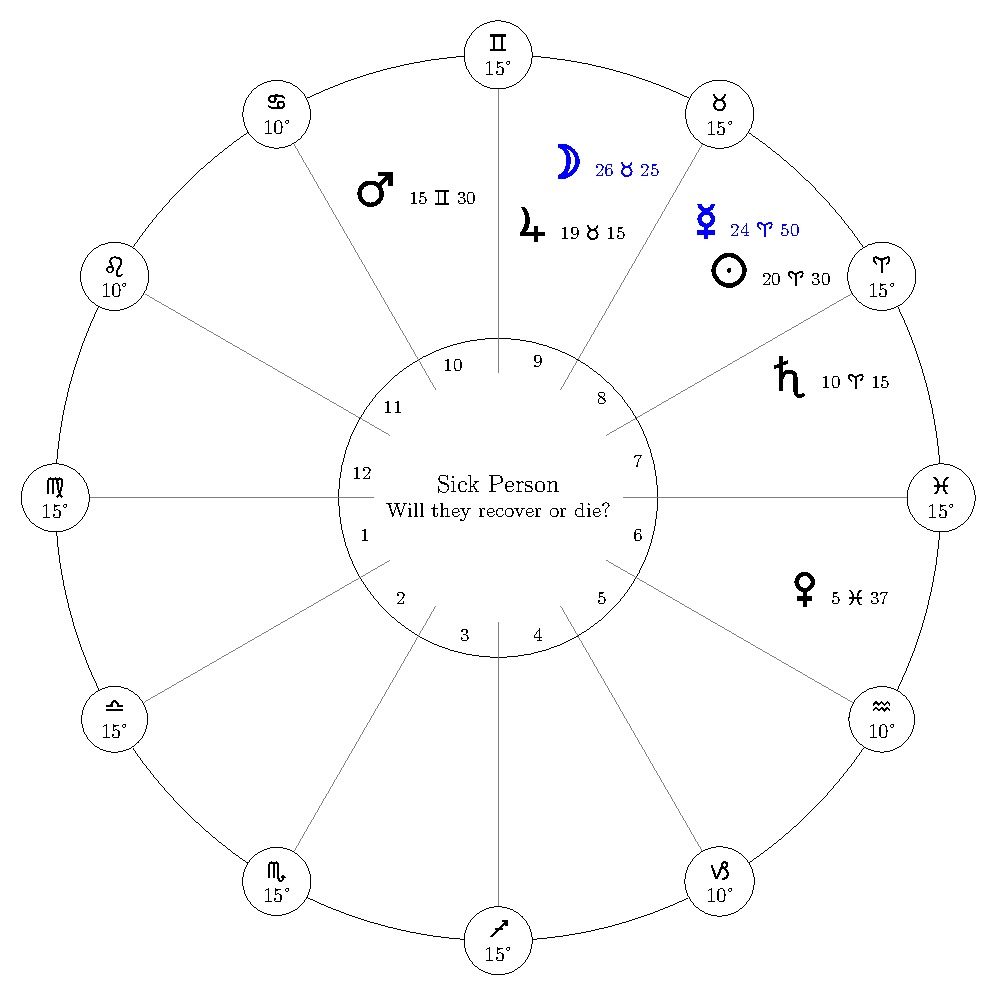
\includegraphics[width=0.9\textwidth]{charts/21-chart-sickness}} \\
\end{center}
\end{columns}

\end{frame}
% ------------------------------------------------------------
\begin{frame}[t]{Sickness Continued}
\begin{columns}[T, onlytextwidth]
\column{0.5\textwidth}
We look at the \Moon, the stronger significator, first. \\
\vspace{0.2cm}
\textbf{\Moon\ in \Taurus\ \Trine\ 1st House} enters \Gemini \\
$\Rightarrow$ \Square\ \Venus\ (in 6th, sickness)  \\
\Venus\ $\Rightarrow$ \Sextile\ \Jupiter, MR by domicile \\

\vspace{0.2cm}
As \Jupiter\ cannot join with any other planet\footnotemark[1], he ends the disposition and becomes the final authority over the matter and so determines the final outcome.

\vspace{0.2cm}
After examining the \Moon\ committing her disposition, Masha'allah looks at \Mercury\ (L1) as sharing in the matter and finds it confirms what the \Moon\ signified.



\column{0.5\textwidth}
\begin{center}
{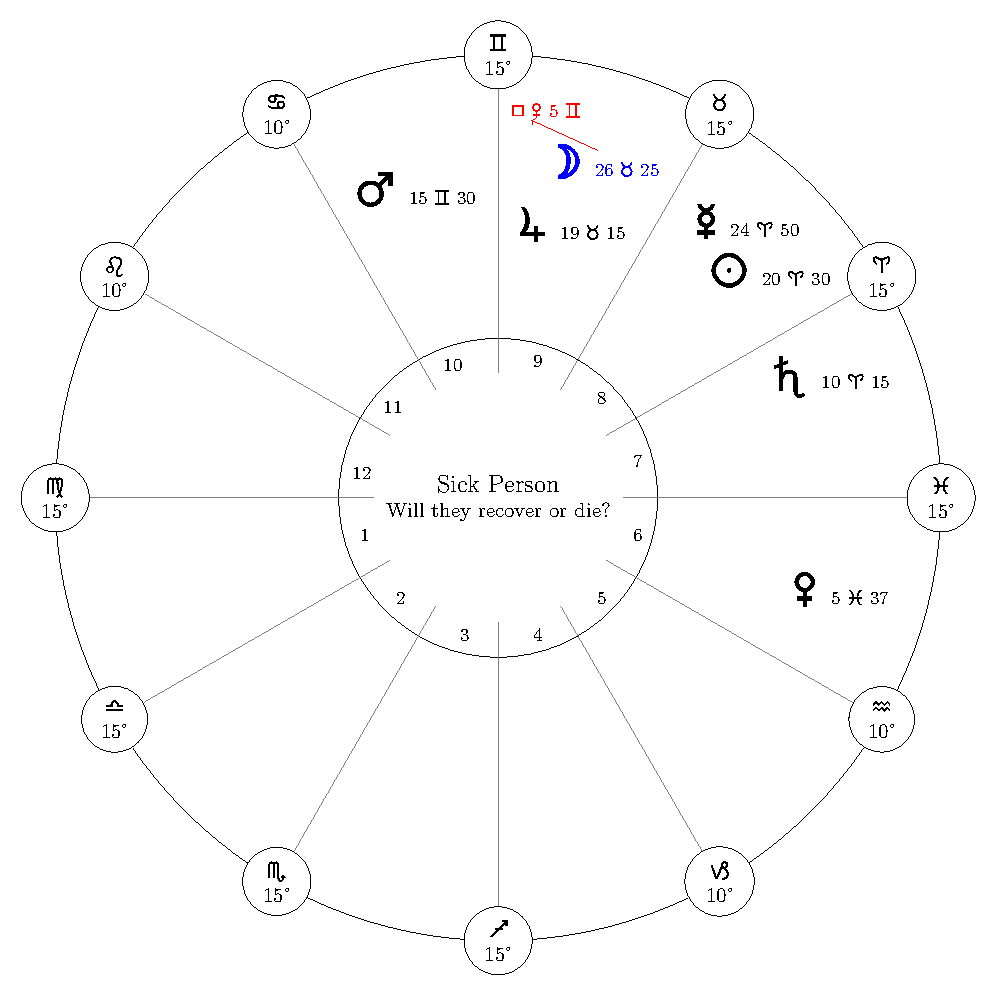
\includegraphics[width=0.9\textwidth]{charts/21a-chart-sickness}} \\
\vspace{-0.2cm}
\end{center}
\end{columns}
\footnotetext[1]{He can only apply to \Saturn\ and he is already separated from him.}
\end{frame}
% ------------------------------------------------------------
\begin{frame}[t]{Sickness Continued}
\begin{columns}[T, onlytextwidth]
\column{0.5\textwidth}

\textbf{\Mercury\ in \Aries\ Void of Course} $\Rightarrow$ \Taurus \\
$\Rightarrow$ \Sextile\ \Venus\ in \Taurus\ accepts his disposition\footnotemark[1] \\
\Venus\ $\Rightarrow$ \Sextile\ \Jupiter\ in \Taurus\, MR by domicile \\
And again, \Jupiter\ is the end of the disposition chain, supporting what the \Moon\ indicated.
\vspace{0.2cm}

\Jupiter, a benefic, as the final arbiter of the disposition promises "health and quiet" and the end of the illness after a prolonged period (due to the VOC's) but we are told that from the time of \Venus\ accepting the \Moon's disposition to her (\Venus's) joining with \Jupiter\ by \Sextile, the person would have gradually strengthened, with the illness leaving him completely once \Venus\ separates from \Jupiter\ by one minute.

\column{0.5\textwidth}
\begin{center}
{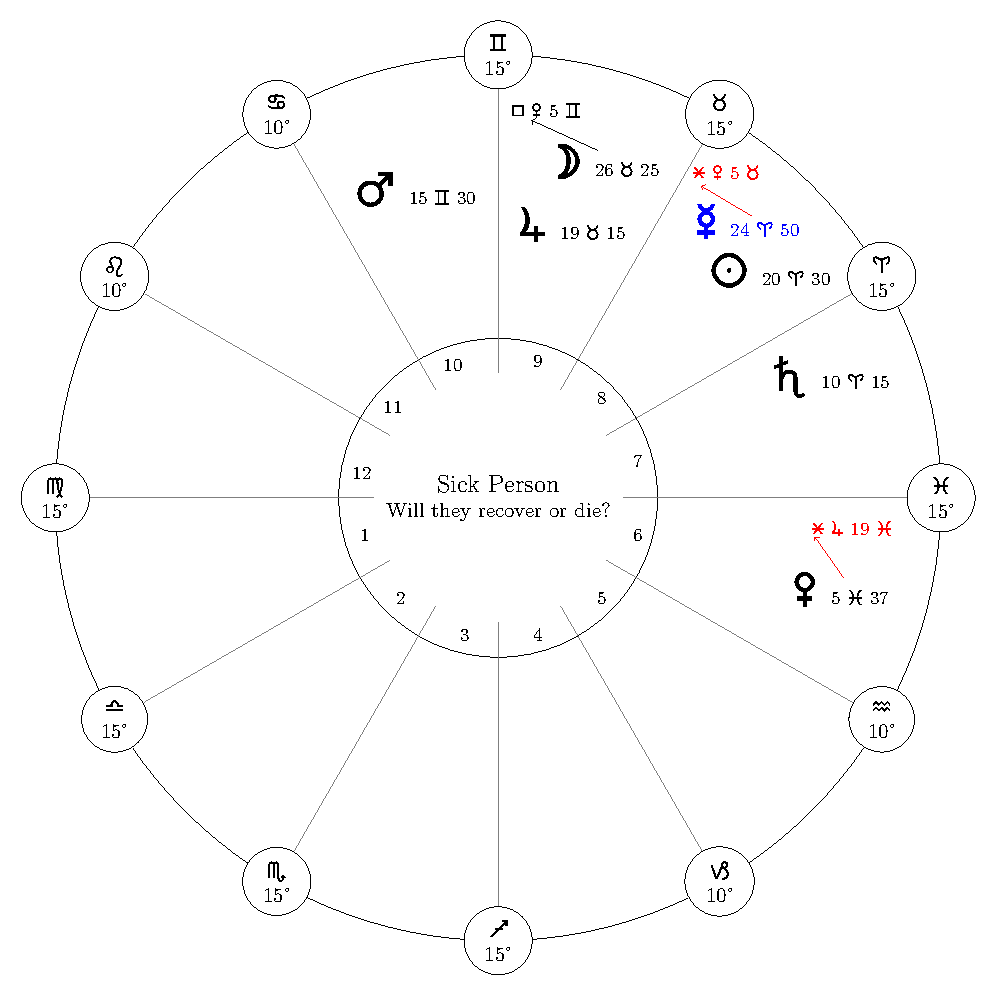
\includegraphics[width=0.9\textwidth]{charts/21b-chart-sickness}} \\
\vspace{-0.2cm}
\end{center}
\end{columns}
\footnotetext[1]{Sahl's mode 14.2, \textsl{Strength of the Planets}, says a planet in dignity can effectively accept a disposition; here it appears to apply to the location of the aspect but it could also apply because \Venus\ has dignity in her place, in \Pisces.}
\end{frame}
% -------------------------------------------------------------------------
\begin{frame}[t]{Sickness (Alternative Scenarios)}
The significator of the matter being asked about (death) is actually \Mars\ as the ruler of the 8th. Masha'allah does list a \Mars\ connection as an alternative scenario, saying such a connection would have meant death for the querent as \Mars's is L8 and does not receive \Venus\ in \Pisces. However, as neither L1 nor the \Moon\ joined to \Mars, the person did not die; although they had a severe illness (\Venus, while not the ruler of the 6th, is in the 6th of sickness). (\textbf{Note:} the \Moon, as the main significator of the querent, is averse to (\Semisextile) \Mars.)\\

\vspace{0.2cm}
He also goes on to warn that had the \Moon\ joined with the \Sun, as he is not L1, he can destroy by combustion if he does not receive the planet, and this also applies to his \Square\ or \Opposition. [JH p23.]\footnotemark[1]

\footnotetext[1]{I've seen this before as a planet being protected from combustion if they are in their own signs; here, the \Moon\ is in her Exaltation but we are told she has to be in the \Sun's signs (\Leo\ or \Aries) to be protected from combustion.}
\end{frame}
\subsection{Example Chart: LIfe Question}
\begin{frame}[t]{Example Chart: Life Question}
\begin{columns}[T, onlytextwidth]
\column{0.5\textwidth}

\column{0.5\textwidth}
\begin{center}
{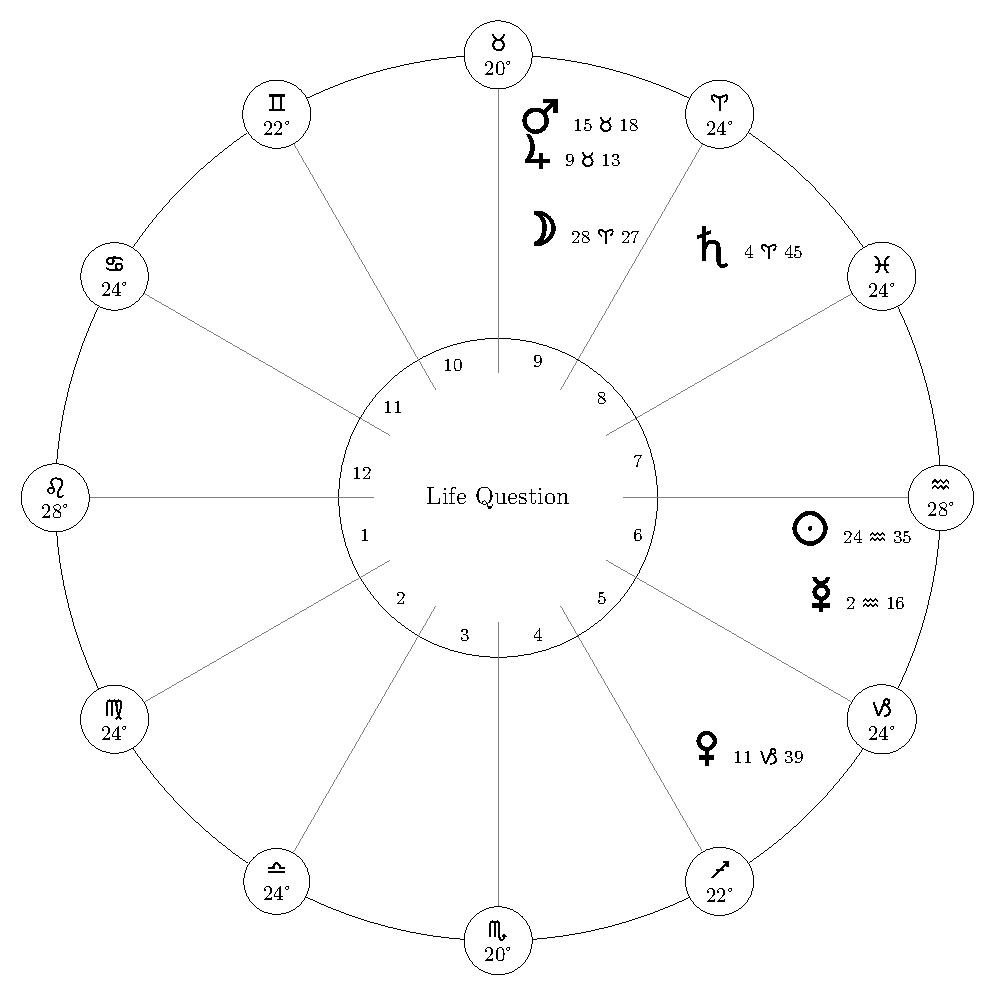
\includegraphics[width=0.9\textwidth]{charts/22-chart-life}}
\end{center}
\end{columns}
\end{frame}

\subsection{Finding Wealth or Not}
\begin{frame}[t]{Finding Wealth or Not [JH 29-31][RH 23-25]}
If the question is about wealth in general, and not specific to some source or person, examine L1 and the \Moon\ to see which is the main significator of the querent and which the sharer and use L2 as the significator of the quesited, wealth.

\begin{block}{}
\textsl{"The connection of the ruler of the Asc or the \Moon\ with the ruler of the thing is the attainment of the thing by itself"}, whether joined to a benefic or malefic, with or without reception, \underline{unless} the significator of the quesited commits its disposition to another planet.\footnotemark[1]
\end{block}

If L2 commits its disposition to:
\begin{itemize}
\item a malefic, with reception, \textsl{"the thing will be perfected"}
\item a benefic, with or without reception, \textsl{"he will find wealth...if the dispositor is in a strong [place] or in the angles"} as angles are useful to the 2nd and hasten things; cadent houses delay things
\end{itemize}

Wealth is also shown if the 2nd holds: a benefic, a dignified malefic, or a malefic without dignity that receives L1.

\footnotetext[1]{Hand says this is true only for the stronger of the two, L1 or \Moon.}
\end{frame}
% -----------------------------------------------
\begin{frame}[t]{Finding Wealth or Not Continued}
If L1 joins with L2 or planets in the 2nd, the querent has been seeking wealth but if L2 joins with L1, the wealth will come about without any seeking on the querent's part and they will receive more than they hoped for.

\textbf{If no L1, \Moon, 2nd House Connections}

If L1 or the \Moon\ do not connect to L2 or a planet in the 2nd, see if one of them connects to a benefic (with or without reception) that is in a strong place or angular; if that benefic does not commit its disposition elsewhere, the querent will find wealth. 

And the same applies if it connects to a malefic with reception but if it is without reception, the matter will be destroyed.

\begin{block}{}
A benefic that commits its disposition to a malefic who does not receive it signifies the matter ruled by the benefic will be harmed when the disposition is complete; with reception, the matter is perfected without harm.
\end{block}

\end{frame}
\subsection{Looking to Borrow}
\begin{frame}[t]{Looking to Borrow}
If a person is looking to borrow from another, L1 and the \Moon\ signify the querent, L2, his wealth while L7 and L8 signify the possible lender and their wealth.

The querent will get what he seeks if:
\begin{itemize}
\item L1 or the \Moon\ are joined to L8 or a planet in the 8th
\item L8 is joined to L1 or a planet in the 1st that is a benefic, a dignified malefic, or a malefic that receives it
\item either  L1 or the \Moon\ is joined to a malefic with reception or a benefic in a strong place
\end{itemize}

But if the person is looking to borrow from the King, use the 11th (Wealth of the King) instead of the 8th.

\end{frame}

\subsection{Inheritance}
\begin{frame}[t]{Inheritance [JH p34] [RH p30]}
\begin{columns}[T, onlytextwidth]
\column{0.5\textwidth}
L1, \Venus\ (16 \Aquarius), was VOC, separating from \Square\  \Jupiter\ (14 \Taurus), L8 (the deceased person's wealth) with reception
\begin{block}{}
\textsl{"Separation by reception is something foul and a horrible thing" [JH 35]}
\end{block}
\Moon\ (28 \Leo) VOC separating from \Opposition\ \Venus\ (16 \Aquarius) \\
\Moon\ first to leave her sign \Leo\ $\Rightarrow$ \Virgo \\
$\Rightarrow$ \Square\ \Mars\ (6 \Virgo), neither planet receives the other, and \\
since \Mars\ is not L8 he signifies prohibition \\
\vspace{0.25cm}
\Venus\ moves from \Aquarius\ to \Pisces \\
$\Rightarrow$ \Square\ \Mars\ (6 \Pisces), neither planet receives the other \\
shows the same as the \Moon; no inheritance

\column{0.5\textwidth}
\begin{center}
{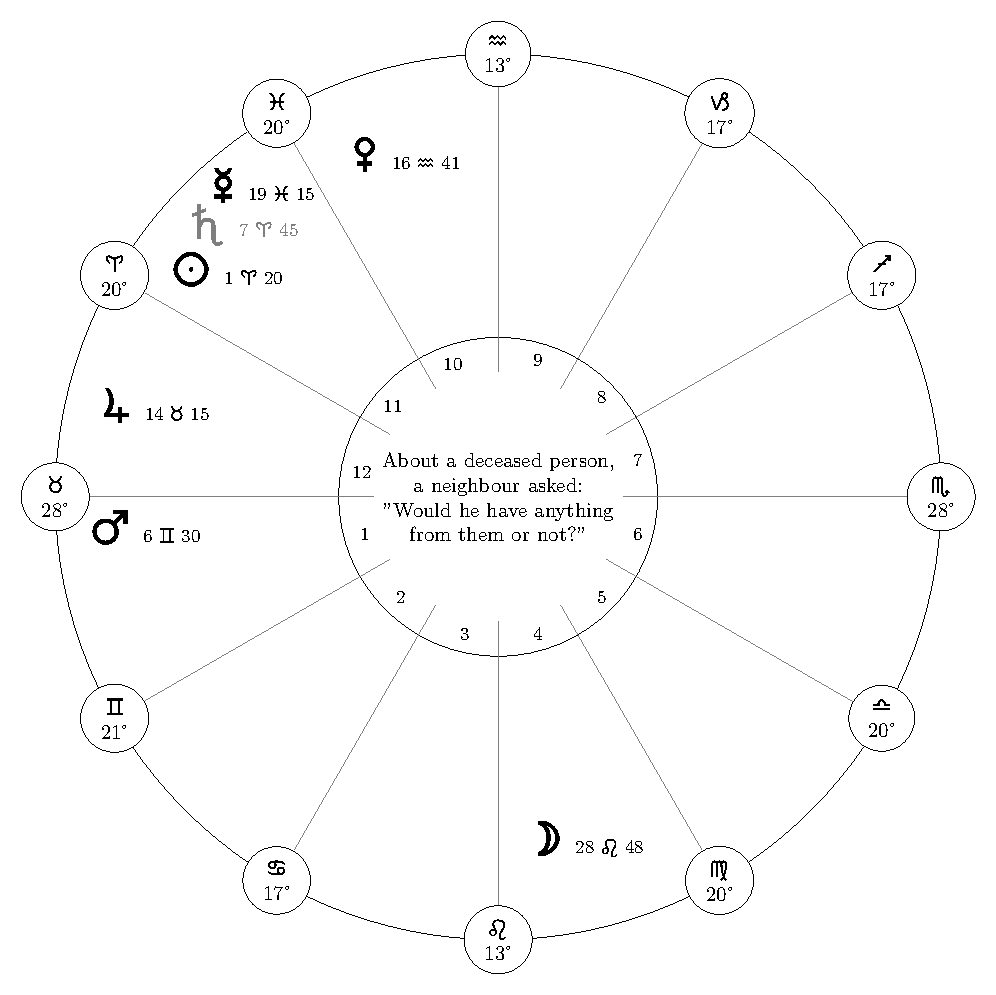
\includegraphics[width=0.9\textwidth]{charts/40-chart-inheritance}} \\
\small
House cusps are not original, Holden shows \Mercury\ at 20 \Pisces; Hand has it at 19 \Pisces\ 15 in the 10th
\end{center}
\end{columns}
\end{frame}

\subsection{Kingdom}
\begin{frame}[t]{Seeking a Kingdom}
\begin{columns}[T, onlytextwidth]
\column{0.5\textwidth}
\Mercury\Retrograde (L1) $\Rightarrow$ \Conjunction\Sun\ $\Rightarrow$ \Sextile\ \Saturn\ (L10) \\
however \\
\Mars\ $\Rightarrow$ \Square\ \Saturn\ (L10) perfects first \\
cutting off the \Sun\ and denying the querent the kingdom \\
\vspace{0.25cm}
And Masha'Allah said the querent would know his hope was lost when \Mars\ perfected its \Square\ to \Saturn \\
\vspace{0.25cm}

Note that the \Moon\ shows the same thing as she first applies to \Mercury, committing her disposition to him and so he hands both his own and her disposition to the the \Sun. And
while  \Mercury\ receives the \Sun, the \Sun\ is not L10 so the matter at hand is not perfected. \\


\column{0.5\textwidth}
\begin{center}
{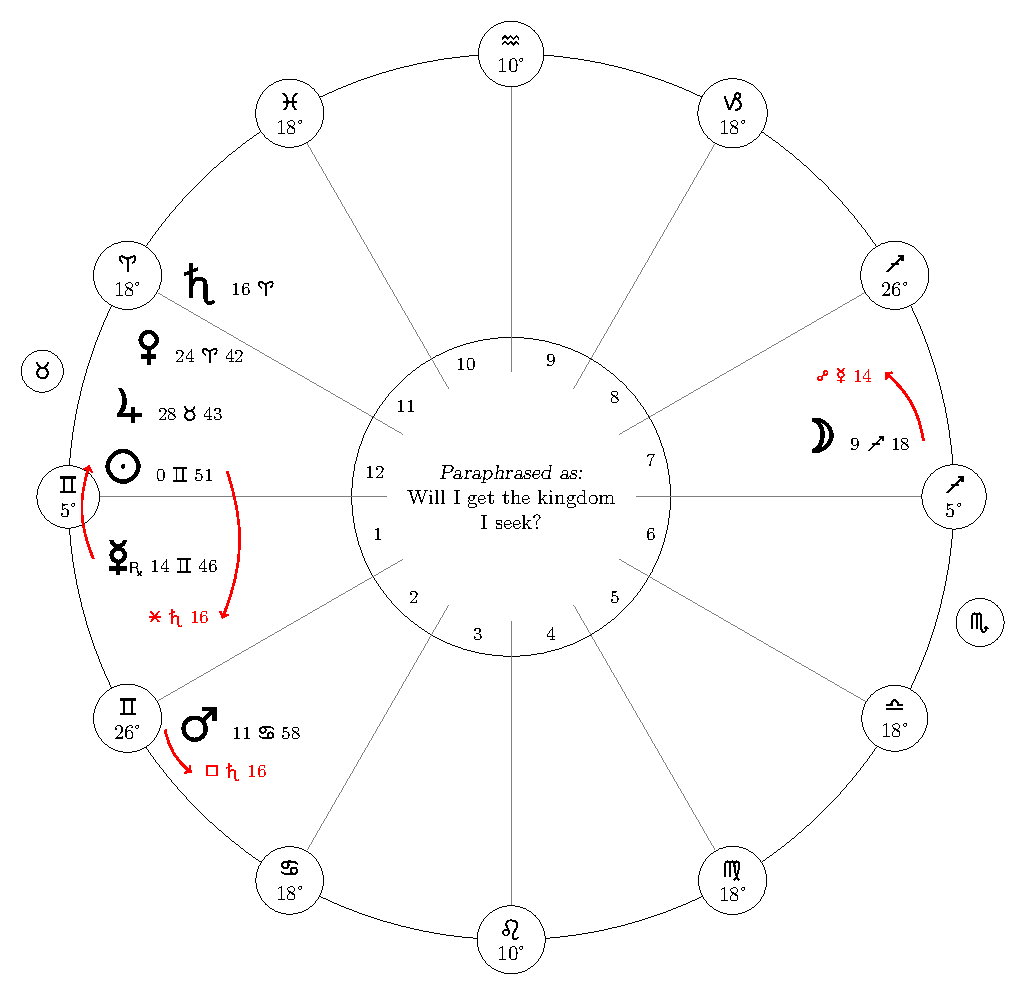
\includegraphics[width=0.9\textwidth]{charts/50-chart-kingdom}} \\
\end{center}
\end{columns}
\end{frame}
% -------------------------------------------------------------------
\begin{frame}[t]{Another Question on a Kingdom}
\begin{columns}[T, onlytextwidth]
\column{0.5\textwidth}
\Moon\ 4 \Libra\ (L1) $\Rightarrow$ \Opposition\ \Saturn\ 11 \Aries\ in the 10th \textsl{"completes"} the matter as \Saturn\ receives the \Moon\ in his exaltation. \\
\vspace{0.5cm}
The man had little joy from his advancement; however, because \Saturn\ was in a place where he had no dignity, being in his Fall and furthermore, in a pitted degree and because it hated its own place it gave something hateful but it made what it gave fixed, strong, and stable because it was in an angle.
 
\column{0.5\textwidth}
\begin{center}
{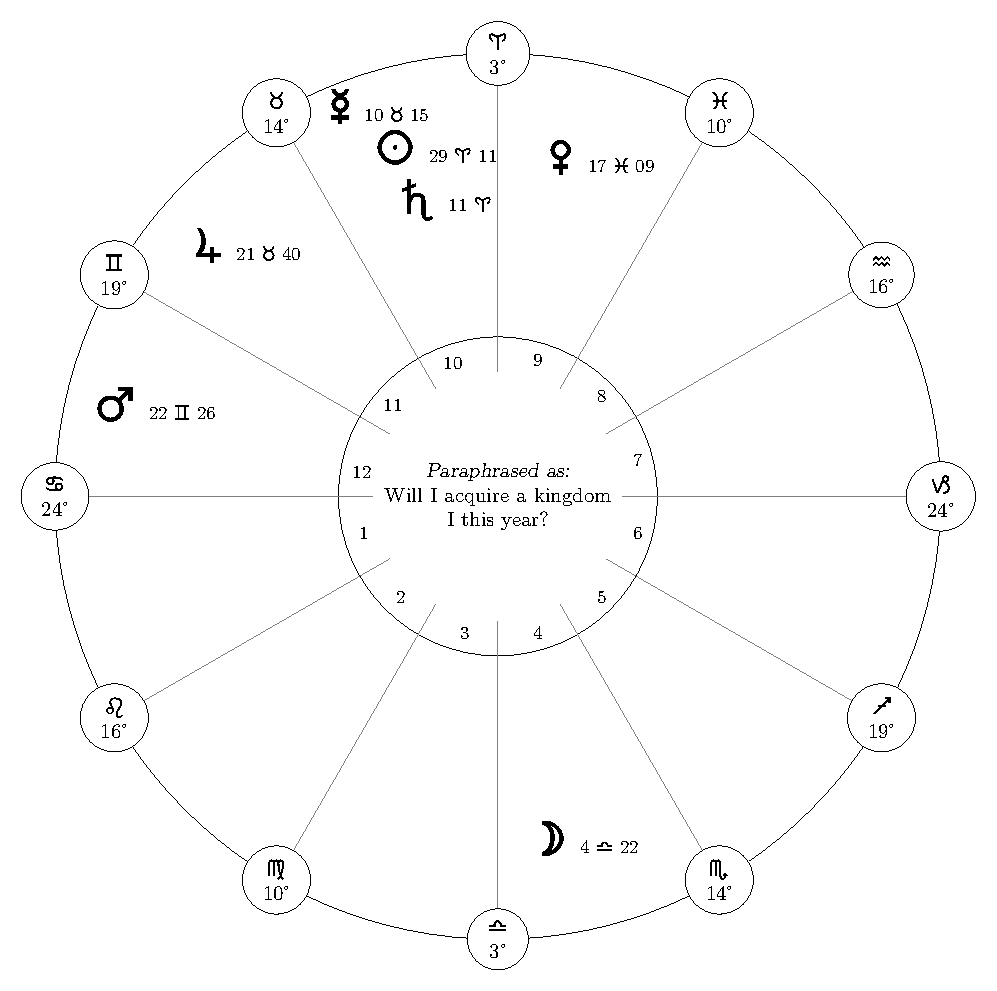
\includegraphics[width=0.9\textwidth]{charts/50-chart-kingdom-1}} \\
\end{center}
\end{columns}
\end{frame}
\input{51-another-kingdom}
\subsection{Will I get the dukedom promised by the King?}
\begin{frame}[t]{Will I get the dukedom promised by the King?}
\begin{columns}[T, onlytextwidth]
\column{0.5\textwidth}
\Jupiter\ is L1, direct, in the 10th (most elevated planet) \\
\hspace{1em}\Sun\ \& \Venus\ $\Rightarrow$ \Square\ from \Sagittarius\ on 1st (received) \\
\hspace{1em}aspects both his domiciles \Sagittarius\ (1st) and \Pisces\ (4th) \\
\hspace{1em}aspects the 7th (connections to all 4 angles) \\
\hspace{1em}signifying he will get his dukedom\\
\vspace{0.5em}
\Mercury\ is L7, retro, a rebel opponent in the matter \\
\hspace{1em}cadent in the 12th \\
\hspace{1em}$\Rightarrow$ \Opposition\ \Saturn\ retro, cadent in 6th\footnotemark[1] (no reception) \\
\hspace{1em}dispositor, \Venus, is combust, worsening matters \\
\hspace{1em}indicates destruction for the opponent \\
\vspace{0.5em}
\Mercury\ retro, by transit, $\Rightarrow$ \Sextile\ \Jupiter\ with reception indicates the rebel opponent will end by seeking "peace and accommodation" from the querent

\column{0.5\textwidth}
\begin{center}
{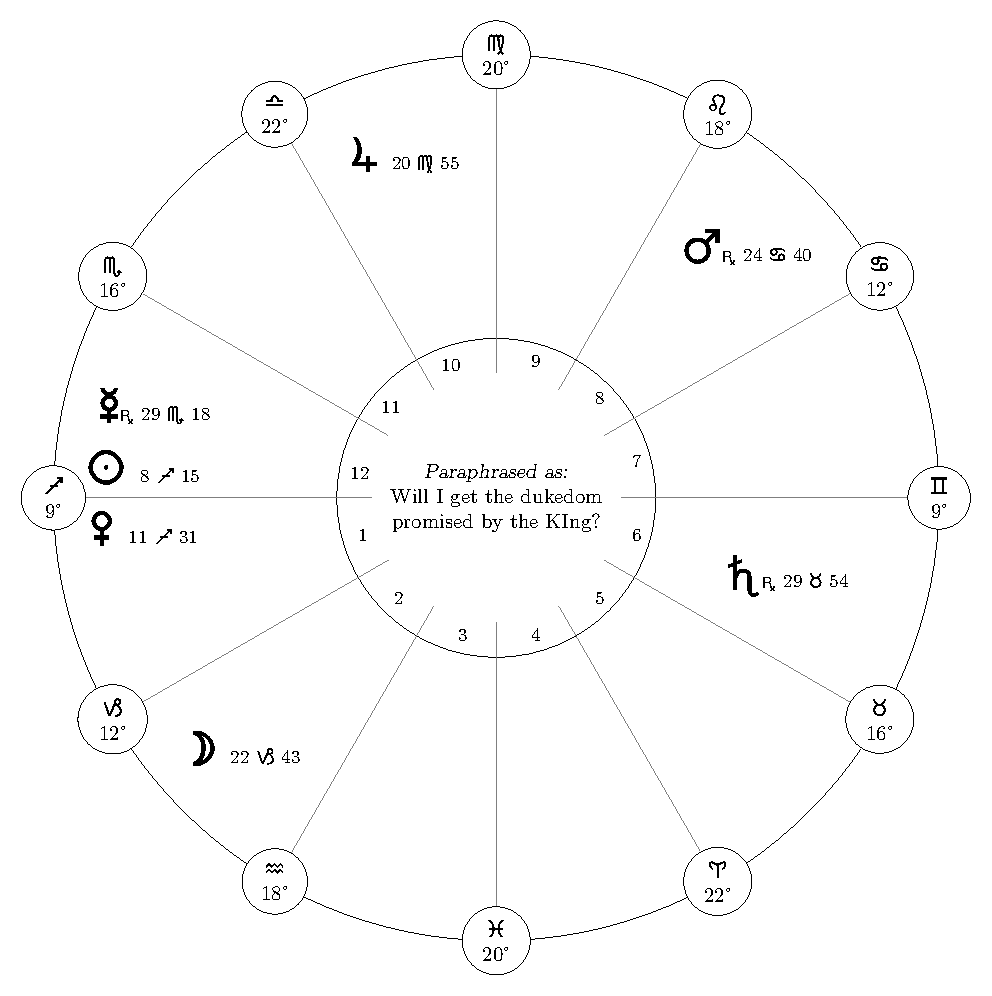
\includegraphics[width=0.9\textwidth]{charts/52-chart-dukedom}} \\
\scriptsize
The MC was not given, only the Asc degree. The other cusps are in the text Holden used but are not original to Masha'Allah.
\end{center}
\end{columns}
\footnotetext[1]{Hand notes this can only be true by Primary Direction.}

\end{frame}
% --------------------------------------------------------------
\begin{frame}[t]{Dukedom Chart as Battle Chart}
Masha'allah goes further into the chart, reading it as a 'battle' or 'war' chart; he begins with the \Moon, using its separating to identify the querent and its application to identify the rebel lord. \\
\vspace{0.25cm}
\Jupiter\ in \Virgo\ \Trine\ (not rec'd) $\Leftarrow$ \Moon\ in \Capricorn\ $\Rightarrow$ \Opposition\ \Mars\ in \Cancer\ (mixed reception) \\
\hspace{1em}\Moon\ is significator of the opponent  in the 2nd (support for querent) \\
\hspace{1em}\Mars\ retro, in 8th, in his Fall; indicating the opponents penury (8th is 2nd from 7th) \\
\hspace{1em} Masha'allah says this indicates the rebel lord could not pay his army \\
\hspace{1em} so the querent bought them off; ending the battle \\
\vspace{0.25cm}
But, as \Mars\ is the dispositor of \Mercury\ (L7), and it is in a strong reception with the \Moon, the rebel lord will not lose everything and, as already noted, \Mercury's \Sextile\ to \Jupiter\ indicates a peaceful conclusion for all involved.

This is the last of Masha'allah's examples.

\end{frame}

\section{Sahl Examples}
\begin{frame}[t]{Translation of Light  - A Question of Marriage}
\begin{columns}[T, onlytextwidth]
\column{0.5\textwidth}
\Mercury\ (L1) (querent) \Quincunx\ \Jupiter\ (L7) (marriage) \\
\Moon\ separating \Sextile\ \Mercury\ applying \Square\ \Jupiter \\
\vspace{0.25cm}
Therefore, the \Moon\ was carrying the light of \Mercury\ to \Jupiter\ \textsl{"and this signified the completion of the thing, i.e. the attainment of the woman through the hands of go-betweens and those running back and forth between the two [parties]."} ([JH] p14-15) \\
\vspace{0.15cm}
\textbf{Note:} \\
\small
In this example, it would seem that the \Moon\ is really the querent's significator as \Mercury\ does not aspect the 1st house nor does he aspect \Jupiter. \\

Looking at the \Moon\ \Sextile\ \Mercury\, could the \Mercury\ reception be of a 'pushing nature' variety? with \Mercury\ doing the pushing rather than the applying \Moon\, who does not receive \Mercury?\footnotemark[1]

\column{0.5\textwidth}
\begin{center}
{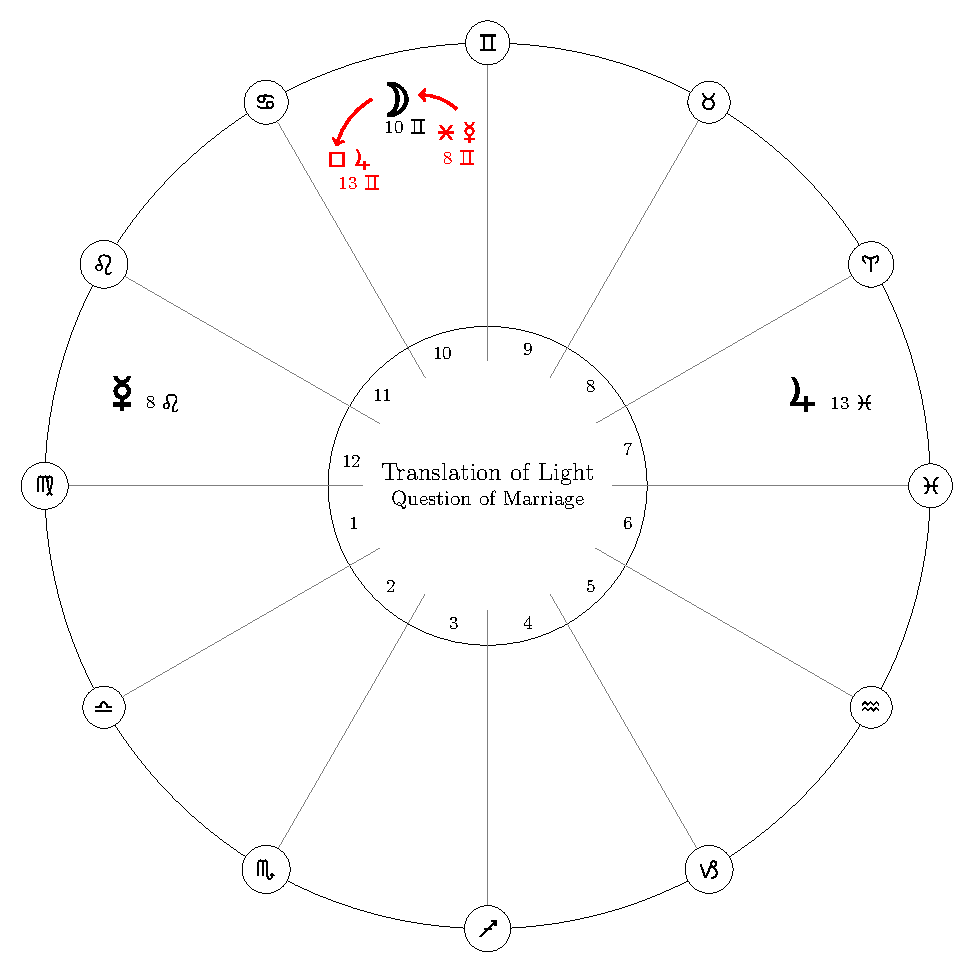
\includegraphics[width=0.9\textwidth]{charts/60-translation}} \\
\end{center}
\end{columns}
\footnotetext[1]{Ibn Ezra "conferring of nature" p121}
\end{frame}

\end{document}